\documentclass{book}
\usepackage[a4paper,top=2.5cm,bottom=2.5cm,left=2.5cm,right=2.5cm]{geometry}
\usepackage{makeidx}
\usepackage{natbib}
\usepackage{graphicx}
\usepackage{multicol}
\usepackage{float}
\usepackage{listings}
\usepackage{color}
\usepackage{ifthen}
\usepackage[table]{xcolor}
\usepackage{textcomp}
\usepackage{alltt}
\usepackage{ifpdf}
\ifpdf
\usepackage[pdftex,
            pagebackref=true,
            colorlinks=true,
            linkcolor=blue,
            unicode
           ]{hyperref}
\else
\usepackage[ps2pdf,
            pagebackref=true,
            colorlinks=true,
            linkcolor=blue,
            unicode
           ]{hyperref}
\usepackage{pspicture}
\fi
\usepackage[utf8]{inputenc}
\usepackage[brazil]{babel}
\usepackage{mathptmx}
\usepackage[scaled=.90]{helvet}
\usepackage{courier}
\usepackage{sectsty}
\usepackage[titles]{tocloft}
\usepackage{doxygen}
\lstset{language=C++,inputencoding=utf8,basicstyle=\footnotesize,breaklines=true,breakatwhitespace=true,tabsize=8,numbers=left }
\makeindex
\setcounter{tocdepth}{3}
\renewcommand{\footrulewidth}{0.4pt}
\renewcommand{\familydefault}{\sfdefault}
\hfuzz=15pt
\setlength{\emergencystretch}{15pt}
\hbadness=750
\tolerance=750
\begin{document}
\hypersetup{pageanchor=false,citecolor=blue}
\begin{titlepage}
\vspace*{7cm}
\begin{center}
{\Large Gunther's Quest Alpha \\[1ex]\large 0.\-2 }\\
\vspace*{1cm}
{\large Gerado por Doxygen 1.8.0}\\
\vspace*{0.5cm}
{\small Domingo, 17 de Junho de 2012 23:27:58}\\
\end{center}
\end{titlepage}
\clearemptydoublepage
\pagenumbering{roman}
\tableofcontents
\clearemptydoublepage
\pagenumbering{arabic}
\hypersetup{pageanchor=true,citecolor=blue}
\chapter{Índice das Estruturas de Dados}
\section{Estruturas de Dados}
Aqui estão as estruturas de dados, uniões e suas respectivas descrições\-:\begin{DoxyCompactList}
\item\contentsline{section}{\hyperlink{struct__jogador}{\-\_\-jogador} }{\pageref{struct__jogador}}{}
\item\contentsline{section}{\hyperlink{struct__ladrilho}{\-\_\-ladrilho} }{\pageref{struct__ladrilho}}{}
\item\contentsline{section}{\hyperlink{struct__objeto}{\-\_\-objeto} }{\pageref{struct__objeto}}{}
\item\contentsline{section}{\hyperlink{struct__tabuleiro}{\-\_\-tabuleiro} }{\pageref{struct__tabuleiro}}{}
\item\contentsline{section}{\hyperlink{structstruct__objeto}{struct\-\_\-objeto} }{\pageref{structstruct__objeto}}{}
\item\contentsline{section}{\hyperlink{structstruct__vetor}{struct\-\_\-vetor} }{\pageref{structstruct__vetor}}{}
\end{DoxyCompactList}

\chapter{Índice dos Arquivos}
\section{Lista de Arquivos}
Esta é a lista de todos os arquivos documentados e suas respectivas descrições\-:\begin{DoxyCompactList}
\item\contentsline{section}{include/\hyperlink{gunther_8h}{gunther.\-h} \\*Arquivo header geral do jogo }{\pageref{gunther_8h}}{}
\item\contentsline{section}{include/\hyperlink{rkefisica_8h}{rkefisica.\-h} \\*Arquivo header da biblioteca de funções físicas }{\pageref{rkefisica_8h}}{}
\item\contentsline{section}{include/\hyperlink{rkegraficos_8h}{rkegraficos.\-h} \\*Arquivo header da parte gráfica }{\pageref{rkegraficos_8h}}{}
\item\contentsline{section}{include/\hyperlink{rkerender_8h}{rkerender.\-h} \\*Arquivo header do renderizador }{\pageref{rkerender_8h}}{}
\item\contentsline{section}{include/\hyperlink{rketypes_8h}{rketypes.\-h} \\*Arquivo header de tipos e defines do Red Knife Engine }{\pageref{rketypes_8h}}{}
\item\contentsline{section}{src/\hyperlink{main_8c}{main.\-c} \\*Ponto de entrada do jogo }{\pageref{main_8c}}{}
\item\contentsline{section}{src/menu/\hyperlink{menu_8c}{menu.\-c} \\*Implementação do menu principal }{\pageref{menu_8c}}{}
\item\contentsline{section}{src/rkegraficos/\hyperlink{rkegraficos_8c}{rkegraficos.\-c} \\*Utilitários gráficos }{\pageref{rkegraficos_8c}}{}
\item\contentsline{section}{src/rkerender/\hyperlink{rkerender_8c}{rkerender.\-c} \\*Renderizador de fases }{\pageref{rkerender_8c}}{}
\end{DoxyCompactList}

\chapter{Estruturas}
\hypertarget{struct__jogador}{
\section{Referência da Estrutura \_\-jogador}
\label{struct__jogador}\index{\_\-jogador@{\_\-jogador}}
}


{\ttfamily \#include $<$player.h$>$}

\subsection*{Campos de Dados}
\begin{DoxyCompactItemize}
\item 
\hypertarget{struct__jogador_a10a4d4bb1fa867a1c3a9bc2ab9ee7e9d}{
SDL\_\-Rect {\bfseries retangulo} \mbox{[}8\mbox{]}}
\label{struct__jogador_a10a4d4bb1fa867a1c3a9bc2ab9ee7e9d}

\item 
\hypertarget{struct__jogador_a6150e0515f7202e2fb518f7206ed97dc}{
int {\bfseries x}}
\label{struct__jogador_a6150e0515f7202e2fb518f7206ed97dc}

\item 
\hypertarget{struct__jogador_a0a2f84ed7838f07779ae24c5a9086d33}{
int {\bfseries y}}
\label{struct__jogador_a0a2f84ed7838f07779ae24c5a9086d33}

\item 
\hypertarget{struct__jogador_a05818f82142eb45301bf89e8939bb8ae}{
int {\bfseries direcao}}
\label{struct__jogador_a05818f82142eb45301bf89e8939bb8ae}

\item 
\hypertarget{struct__jogador_a9aa790f93d2d067a4f5608fdb8409f94}{
int {\bfseries hp}}
\label{struct__jogador_a9aa790f93d2d067a4f5608fdb8409f94}

\item 
\hypertarget{struct__jogador_a5819a445ff2fb05f613477829c04f115}{
int {\bfseries poder\_\-flecha}}
\label{struct__jogador_a5819a445ff2fb05f613477829c04f115}

\item 
\hypertarget{struct__jogador_a7ba2606514453e5bedf98b5510b8169e}{
int {\bfseries poder\_\-bomba}}
\label{struct__jogador_a7ba2606514453e5bedf98b5510b8169e}

\item 
\hypertarget{struct__jogador_a06e0ae6abeebe6c53b256cca1e00fedf}{
int {\bfseries bombas}}
\label{struct__jogador_a06e0ae6abeebe6c53b256cca1e00fedf}

\end{DoxyCompactItemize}


\subsection{Descrição Detalhada}
Struct Jogador 
\begin{DoxyParams}{Parâmetros}
{\em retangulo} & Vetor com os 8 retângulos das visões do jogador \\
\hline
{\em x} & Posição x do jogador \\
\hline
{\em y} & Posição y do jogador \\
\hline
{\em direcao} & Direção que o jogador está olhando \\
\hline
{\em hp} & Quantidade de hp do jogador \\
\hline
\end{DoxyParams}


A documentação para esta estrutura foi gerada a partir do seguinte arquivo:\begin{DoxyCompactItemize}
\item 
\hyperlink{player_8h}{player.h}\end{DoxyCompactItemize}

\hypertarget{struct__ladrilho}{\section{Referência da Estrutura \-\_\-ladrilho}
\label{struct__ladrilho}\index{\-\_\-ladrilho@{\-\_\-ladrilho}}
}


{\ttfamily \#include $<$rkerender.\-h$>$}

\subsection*{Campos de Dados}
\begin{DoxyCompactItemize}
\item 
\hypertarget{struct__ladrilho_a66706353d918fc22d4b7130ef5a9fbc4}{S\-D\-L\-\_\-\-Rect {\bfseries retangulo}}\label{struct__ladrilho_a66706353d918fc22d4b7130ef5a9fbc4}

\item 
\hypertarget{struct__ladrilho_af4541a0087b5e63cdca818a994d5119c}{int {\bfseries passavel}}\label{struct__ladrilho_af4541a0087b5e63cdca818a994d5119c}

\end{DoxyCompactItemize}


\subsection{Descrição Detalhada}
Struct Ladrilho 
\begin{DoxyParams}{Parâmetros}
{\em retangulo} & Retângulo do ladrilho \\
\hline
{\em passavel} & Indica se o jogador pode andar em cima do ladrilho \\
\hline
\end{DoxyParams}


A documentação para esta estrutura foi gerada a partir do seguinte arquivo\-:\begin{DoxyCompactItemize}
\item 
include/\hyperlink{rkerender_8h}{rkerender.\-h}\end{DoxyCompactItemize}

\hypertarget{struct__objeto}{
\section{Referência da Estrutura \_\-objeto}
\label{struct__objeto}\index{\_\-objeto@{\_\-objeto}}
}


{\ttfamily \#include $<$rkerender.h$>$}

\subsection*{Campos de Dados}
\begin{DoxyCompactItemize}
\item 
\hypertarget{struct__objeto_a66706353d918fc22d4b7130ef5a9fbc4}{
SDL\_\-Rect {\bfseries retangulo}}
\label{struct__objeto_a66706353d918fc22d4b7130ef5a9fbc4}

\item 
\hypertarget{struct__objeto_a9aa790f93d2d067a4f5608fdb8409f94}{
int {\bfseries hp}}
\label{struct__objeto_a9aa790f93d2d067a4f5608fdb8409f94}

\item 
\hypertarget{struct__objeto_a7241422808ffa774468b342f39b6ae1f}{
int {\bfseries attack}}
\label{struct__objeto_a7241422808ffa774468b342f39b6ae1f}

\item 
\hypertarget{struct__objeto_a21a6e1305c3f396d42ee151e8751b469}{
int {\bfseries bonus}}
\label{struct__objeto_a21a6e1305c3f396d42ee151e8751b469}

\end{DoxyCompactItemize}


\subsection{Descrição Detalhada}
Struct Objeto 
\begin{DoxyParams}{Parâmetros}
{\em retangulo} & Retângulo da imagem do objeto no clipboard \\
\hline
{\em hp} & Quantidade de hp do objeto \\
\hline
{\em attack} & Tipo de ataque do objeto \\
\hline
{\em bonus} & Tipo de bonus do objeto \\
\hline
\end{DoxyParams}


A documentação para esta estrutura foi gerada a partir do seguinte arquivo:\begin{DoxyCompactItemize}
\item 
bkp/\hyperlink{rkerender_8h}{rkerender.h}\end{DoxyCompactItemize}

\hypertarget{struct__tabuleiro}{\section{Referência da Estrutura \-\_\-tabuleiro}
\label{struct__tabuleiro}\index{\-\_\-tabuleiro@{\-\_\-tabuleiro}}
}


{\ttfamily \#include $<$rkerender.\-h$>$}

\subsection*{Campos de Dados}
\begin{DoxyCompactItemize}
\item 
\hypertarget{struct__tabuleiro_a769a0d58682f084ffb749f2b7ab745a4}{char $\ast$$\ast$ {\bfseries terreno}}\label{struct__tabuleiro_a769a0d58682f084ffb749f2b7ab745a4}

\item 
\hypertarget{struct__tabuleiro_ab72c9e88a2e860a6183e6264189de9c3}{char $\ast$$\ast$ {\bfseries objetos}}\label{struct__tabuleiro_ab72c9e88a2e860a6183e6264189de9c3}

\end{DoxyCompactItemize}


\subsection{Descrição Detalhada}
Struct Tabuleiro 
\begin{DoxyParams}{Parâmetros}
{\em terreno} & Matriz que armazena como o terreno é construído \\
\hline
{\em objetos} & Matriz que armazena a localização dos objetos \\
\hline
\end{DoxyParams}


A documentação para esta estrutura foi gerada a partir do seguinte arquivo\-:\begin{DoxyCompactItemize}
\item 
include/\hyperlink{rkerender_8h}{rkerender.\-h}\end{DoxyCompactItemize}

\hypertarget{structstruct__objeto}{\section{Referência da Estrutura struct\-\_\-objeto}
\label{structstruct__objeto}\index{struct\-\_\-objeto@{struct\-\_\-objeto}}
}


{\ttfamily \#include $<$rketypes.\-h$>$}

\subsection*{Campos de Dados}
\begin{DoxyCompactItemize}
\item 
\hypertarget{structstruct__objeto_a7441ef0865bcb3db9b8064dd7375c1ea}{int {\bfseries id}}\label{structstruct__objeto_a7441ef0865bcb3db9b8064dd7375c1ea}

\item 
\hypertarget{structstruct__objeto_af88b946fb90d5f08b5fb740c70e98c10}{double {\bfseries x}}\label{structstruct__objeto_af88b946fb90d5f08b5fb740c70e98c10}

\item 
\hypertarget{structstruct__objeto_ab927965981178aa1fba979a37168db2a}{double {\bfseries y}}\label{structstruct__objeto_ab927965981178aa1fba979a37168db2a}

\item 
\hypertarget{structstruct__objeto_af8ea4d2851d2d656fd42be239e36ce6e}{double {\bfseries v\-\_\-x}}\label{structstruct__objeto_af8ea4d2851d2d656fd42be239e36ce6e}

\item 
\hypertarget{structstruct__objeto_a2161079bbf87834cfdf4d3548a53eb3b}{double {\bfseries v\-\_\-y}}\label{structstruct__objeto_a2161079bbf87834cfdf4d3548a53eb3b}

\item 
\hypertarget{structstruct__objeto_a3cb08d781a7ecc13047f1631906f7df5}{double {\bfseries massa}}\label{structstruct__objeto_a3cb08d781a7ecc13047f1631906f7df5}

\item 
\hypertarget{structstruct__objeto_aff2f6d52166217d13f9b2072c9e67c13}{double {\bfseries tempo}}\label{structstruct__objeto_aff2f6d52166217d13f9b2072c9e67c13}

\end{DoxyCompactItemize}


\subsection{Descrição Detalhada}
Struct objeto 
\begin{DoxyParams}{Parâmetros}
{\em id} & Identificador único \\
\hline
{\em x} & Componente x \\
\hline
{\em y} & Componente y \\
\hline
{\em v\-\_\-x} & Componente x da velocidade do objeto \\
\hline
{\em v\-\_\-y} & Componente y da velocidade do objeto \\
\hline
{\em massa} & Massa do objeto \\
\hline
{\em tempo} & Tempo de vida do objeto \\
\hline
\end{DoxyParams}


A documentação para esta estrutura foi gerada a partir do seguinte arquivo\-:\begin{DoxyCompactItemize}
\item 
include/\hyperlink{rketypes_8h}{rketypes.\-h}\end{DoxyCompactItemize}

\hypertarget{structstruct__vetor}{\section{struct\-\_\-vetor Struct Reference}
\label{structstruct__vetor}\index{struct\-\_\-vetor@{struct\-\_\-vetor}}
}


{\ttfamily \#include $<$rketypes.\-h$>$}

\subsection*{Public Attributes}
\begin{DoxyCompactItemize}
\item 
\hypertarget{structstruct__vetor_aae7646e904a8ce82b9c179ee26a0cc76}{double {\bfseries x}}\label{structstruct__vetor_aae7646e904a8ce82b9c179ee26a0cc76}

\item 
\hypertarget{structstruct__vetor_a73fafc2561b7eb18209e5ee4f6837b28}{double {\bfseries y}}\label{structstruct__vetor_a73fafc2561b7eb18209e5ee4f6837b28}

\end{DoxyCompactItemize}


\subsection{Detailed Description}
Struct vetor 
\begin{DoxyParams}{Parameters}
{\em x} & Componente x \\
\hline
{\em y} & Componente y \\
\hline
\end{DoxyParams}


The documentation for this struct was generated from the following file\-:\begin{DoxyCompactItemize}
\item 
include/\hyperlink{rketypes_8h}{rketypes.\-h}\end{DoxyCompactItemize}

\chapter{Arquivos}
\hypertarget{gunther_8h}{
\section{Referência do Arquivo bkp/gunther.h}
\label{gunther_8h}\index{bkp/gunther.h@{bkp/gunther.h}}
}


Arquivo header geral do jogo.  


{\ttfamily \#include $<$SDL/SDL.h$>$}\par
{\ttfamily \#include \char`\"{}rkegraficos.h\char`\"{}}\par
{\ttfamily \#include \char`\"{}rkefisica.h\char`\"{}}\par
{\ttfamily \#include \char`\"{}rkerender.h\char`\"{}}\par
Gráfico de dependência de inclusões para gunther.h:
\nopagebreak
\begin{figure}[H]
\begin{center}
\leavevmode
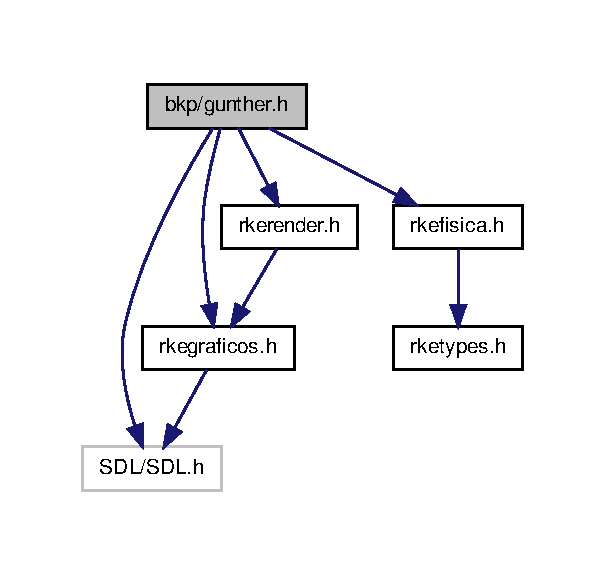
\includegraphics[width=291pt]{gunther_8h__incl}
\end{center}
\end{figure}
Este grafo mostra quais arquivos estão direta ou indiretamente relacionados com este arquivo:
\nopagebreak
\begin{figure}[H]
\begin{center}
\leavevmode
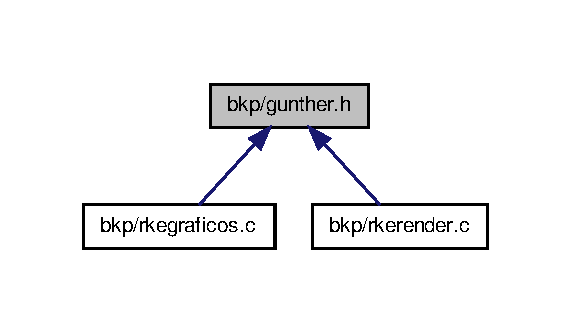
\includegraphics[width=274pt]{gunther_8h__dep__incl}
\end{center}
\end{figure}
\subsection*{Definições e Macros}
\begin{DoxyCompactItemize}
\item 
\hypertarget{gunther_8h_aa29850487e98eb77aec0eb11074210bf}{
\#define {\bfseries DIR\_\-IMAGENS}~\char`\"{}data/imagens/\char`\"{}}
\label{gunther_8h_aa29850487e98eb77aec0eb11074210bf}

\item 
\hypertarget{gunther_8h_a76006c64dff69d69316d1e75795d7fa2}{
\#define {\bfseries LADRILHO\_\-ALTURA}~48}
\label{gunther_8h_a76006c64dff69d69316d1e75795d7fa2}

\item 
\hypertarget{gunther_8h_ac57ee6ff2f62d9fd05e4c636bc432617}{
\#define {\bfseries LADRILHO\_\-LARGURA}~48}
\label{gunther_8h_ac57ee6ff2f62d9fd05e4c636bc432617}

\item 
\hypertarget{gunther_8h_a5c2f746df6889e0255a635c9fff490fe}{
\#define {\bfseries TELA\_\-LARGURA}~15}
\label{gunther_8h_a5c2f746df6889e0255a635c9fff490fe}

\item 
\hypertarget{gunther_8h_a18bb49d2ce68f4af9651cad0173968f0}{
\#define {\bfseries TELA\_\-ALTURA}~10}
\label{gunther_8h_a18bb49d2ce68f4af9651cad0173968f0}

\item 
\hypertarget{gunther_8h_a1ebfd016359b8eecc23a2d3149b11631}{
\#define {\bfseries SAIR}~-\/1}
\label{gunther_8h_a1ebfd016359b8eecc23a2d3149b11631}

\item 
\hypertarget{gunther_8h_a60034ec3e699870774b3424699164ad6}{
\#define {\bfseries NOVOJOGO}~0}
\label{gunther_8h_a60034ec3e699870774b3424699164ad6}

\item 
\hypertarget{gunther_8h_a28bf6e0dbe895b412486bec8741fb84c}{
\#define {\bfseries CARREGAJOGO}~1}
\label{gunther_8h_a28bf6e0dbe895b412486bec8741fb84c}

\item 
\hypertarget{gunther_8h_acbb11be448a8d2fe5244c1a270ae60a5}{
\#define {\bfseries OPCOES}~2}
\label{gunther_8h_acbb11be448a8d2fe5244c1a270ae60a5}

\item 
\hypertarget{gunther_8h_a8187a9af791c0a44ba67edd9cf266961}{
\#define {\bfseries MANUAL}~3}
\label{gunther_8h_a8187a9af791c0a44ba67edd9cf266961}

\item 
\hypertarget{gunther_8h_af1b45216a8f0fae46932075409f7e4c9}{
\#define {\bfseries CREDITOS}~4}
\label{gunther_8h_af1b45216a8f0fae46932075409f7e4c9}

\item 
\hypertarget{gunther_8h_a79b459f7661569a7c189d4279dfb5468}{
\#define {\bfseries INICIO}~5}
\label{gunther_8h_a79b459f7661569a7c189d4279dfb5468}

\item 
\hypertarget{gunther_8h_a1e4a399af19cbd4b1c2fc5f437cddc19}{
\#define {\bfseries COMMANDOS}~6}
\label{gunther_8h_a1e4a399af19cbd4b1c2fc5f437cddc19}

\end{DoxyCompactItemize}
\subsection*{Funções}
\begin{DoxyCompactItemize}
\item 
void \hyperlink{gunther_8h_acf814435dd822e55f2537b49cc6c1505}{gunther\_\-menu} (SDL\_\-Surface $\ast$tela)
\item 
\hypertarget{gunther_8h_ac241ff40fd02c916d3dd71a0f150d3f6}{
int {\bfseries inicio} (SDL\_\-Surface $\ast$screen)}
\label{gunther_8h_ac241ff40fd02c916d3dd71a0f150d3f6}

\item 
int \hyperlink{gunther_8h_af3231d0d69b075fdf6a3fffc4e05f50b}{manual} (SDL\_\-Surface $\ast$screen, int section)
\end{DoxyCompactItemize}


\subsection{Descrição Detalhada}
Arquivo header geral do jogo. \begin{DoxyAuthor}{Autor}
João da Silva, Marina Salles, Ricardo Macedo 
\end{DoxyAuthor}


\subsection{Funções}
\hypertarget{gunther_8h_acf814435dd822e55f2537b49cc6c1505}{
\index{gunther.h@{gunther.h}!gunther\_\-menu@{gunther\_\-menu}}
\index{gunther\_\-menu@{gunther\_\-menu}!gunther.h@{gunther.h}}
\subsubsection[{gunther\_\-menu}]{\setlength{\rightskip}{0pt plus 5cm}void gunther\_\-menu (
\begin{DoxyParamCaption}
\item[{SDL\_\-Surface $\ast$}]{screen}
\end{DoxyParamCaption}
)}}
\label{gunther_8h_acf814435dd822e55f2537b49cc6c1505}
Renderiza o menu baseado na seleção 
\begin{DoxyParams}{Parâmetros}
{\em tela} & Tela onde o menu será renderizado \\
\hline
\end{DoxyParams}
\hypertarget{gunther_8h_af3231d0d69b075fdf6a3fffc4e05f50b}{
\index{gunther.h@{gunther.h}!manual@{manual}}
\index{manual@{manual}!gunther.h@{gunther.h}}
\subsubsection[{manual}]{\setlength{\rightskip}{0pt plus 5cm}int manual (
\begin{DoxyParamCaption}
\item[{SDL\_\-Surface $\ast$}]{screen, }
\item[{int}]{mode}
\end{DoxyParamCaption}
)}}
\label{gunther_8h_af3231d0d69b075fdf6a3fffc4e05f50b}
Seção \char`\"{}Manual\char`\"{} do menu 
\begin{DoxyParams}{Parâmetros}
{\em tela} & Tela onde a seção será renderizada \\
\hline
\end{DoxyParams}

\hypertarget{rkefisica_8h}{\section{Referência do Arquivo include/rkefisica.h}
\label{rkefisica_8h}\index{include/rkefisica.\-h@{include/rkefisica.\-h}}
}


Arquivo header da biblioteca de funções físicas.  


{\ttfamily \#include \char`\"{}rketypes.\-h\char`\"{}}\\*
Gráfico de dependência de inclusões para rkefisica.\-h\-:
Este grafo mostra quais arquivos estão direta ou indiretamente relacionados com este arquivo\-:
\subsection*{Funções}
\begin{DoxyCompactItemize}
\item 
void \hyperlink{rkefisica_8h_ae474cc3a29378896516478d39e1059b9}{rke\-\_\-set\-\_\-delta\-\_\-t} (double d\-\_\-t)
\item 
void \hyperlink{rkefisica_8h_ad9c136c98e2b18bb585f8c5b5c61152e}{rke\-\_\-set\-\_\-arrasto} (double coef\-\_\-arrasto)
\item 
void \hyperlink{rkefisica_8h_a4966d99bd4c2668b7d59a5e334330f86}{rke\-\_\-set\-\_\-vetor\-\_\-mundo} (double x, double y)
\item 
void \hyperlink{rkefisica_8h_ad669b81728dbf96d76dbed56981a3e84}{rke\-\_\-set\-\_\-numero\-\_\-objetos} (int numero)
\item 
void \hyperlink{rkefisica_8h_a4f887533c58a96b4cd5eff48ef195902}{rke\-\_\-adiciona\-\_\-objeto} (int id, double x, double y, double v\-\_\-x, double v\-\_\-y, double massa, double tempo)
\item 
\hyperlink{rketypes_8h_a216693704a51093135790527237245ec}{objeto} \hyperlink{rkefisica_8h_a3db469cd5f289d1376d1d27b53067875}{rke\-\_\-get\-\_\-objeto} (int i)
\item 
int \hyperlink{rkefisica_8h_a1c031c9197d9bfc50cdee27c0d8dd60a}{rke\-\_\-conta\-\_\-objetos} ()
\item 
void \hyperlink{rkefisica_8h_ae68fcd8b02679fe3b05c319820641449}{rke\-\_\-simula} ()
\end{DoxyCompactItemize}


\subsection{Descrição Detalhada}
Arquivo header da biblioteca de funções físicas. \begin{DoxyAuthor}{Autor}
João da Silva, Marina Salles, Ricardo Macedo 
\end{DoxyAuthor}


\subsection{Funções}
\hypertarget{rkefisica_8h_a4f887533c58a96b4cd5eff48ef195902}{\index{rkefisica.\-h@{rkefisica.\-h}!rke\-\_\-adiciona\-\_\-objeto@{rke\-\_\-adiciona\-\_\-objeto}}
\index{rke\-\_\-adiciona\-\_\-objeto@{rke\-\_\-adiciona\-\_\-objeto}!rkefisica.h@{rkefisica.\-h}}
\subsubsection[{rke\-\_\-adiciona\-\_\-objeto}]{\setlength{\rightskip}{0pt plus 5cm}void {\bf rke\-\_\-adiciona\-\_\-objeto} (
\begin{DoxyParamCaption}
\item[{int}]{id, }
\item[{double}]{x, }
\item[{double}]{y, }
\item[{double}]{v\-\_\-x, }
\item[{double}]{v\-\_\-y, }
\item[{double}]{massa, }
\item[{double}]{tempo}
\end{DoxyParamCaption}
)}}\label{rkefisica_8h_a4f887533c58a96b4cd5eff48ef195902}
Adiciona um objeto à lista de objetos a serem simulados. 
\begin{DoxyParams}{Parâmetros}
{\em id} & Identificador único do objeto \\
\hline
{\em x} & Posição x do objeto \\
\hline
{\em y} & Posição y do objeto \\
\hline
{\em v\-\_\-x} & Velocidade em x do objeto \\
\hline
{\em v\-\_\-y} & Velocidade em y do objeto \\
\hline
{\em massa} & Massa do objeto \\
\hline
{\em tempo} & Tempo de vida do objeto em segundos \\
\hline
\end{DoxyParams}
\hypertarget{rkefisica_8h_a1c031c9197d9bfc50cdee27c0d8dd60a}{\index{rkefisica.\-h@{rkefisica.\-h}!rke\-\_\-conta\-\_\-objetos@{rke\-\_\-conta\-\_\-objetos}}
\index{rke\-\_\-conta\-\_\-objetos@{rke\-\_\-conta\-\_\-objetos}!rkefisica.h@{rkefisica.\-h}}
\subsubsection[{rke\-\_\-conta\-\_\-objetos}]{\setlength{\rightskip}{0pt plus 5cm}int {\bf rke\-\_\-conta\-\_\-objetos} (
\begin{DoxyParamCaption}
{}
\end{DoxyParamCaption}
)}}\label{rkefisica_8h_a1c031c9197d9bfc50cdee27c0d8dd60a}
Conta o número de objetos ativos, ou seja, com tempo de vida diferente de zero. \hypertarget{rkefisica_8h_a3db469cd5f289d1376d1d27b53067875}{\index{rkefisica.\-h@{rkefisica.\-h}!rke\-\_\-get\-\_\-objeto@{rke\-\_\-get\-\_\-objeto}}
\index{rke\-\_\-get\-\_\-objeto@{rke\-\_\-get\-\_\-objeto}!rkefisica.h@{rkefisica.\-h}}
\subsubsection[{rke\-\_\-get\-\_\-objeto}]{\setlength{\rightskip}{0pt plus 5cm}{\bf objeto} {\bf rke\-\_\-get\-\_\-objeto} (
\begin{DoxyParamCaption}
\item[{int}]{i}
\end{DoxyParamCaption}
)}}\label{rkefisica_8h_a3db469cd5f289d1376d1d27b53067875}
Retorna o i-\/ésimo objeto. 
\begin{DoxyParams}{Parâmetros}
{\em i} & Índice do objeto \\
\hline
\end{DoxyParams}
\hypertarget{rkefisica_8h_ad9c136c98e2b18bb585f8c5b5c61152e}{\index{rkefisica.\-h@{rkefisica.\-h}!rke\-\_\-set\-\_\-arrasto@{rke\-\_\-set\-\_\-arrasto}}
\index{rke\-\_\-set\-\_\-arrasto@{rke\-\_\-set\-\_\-arrasto}!rkefisica.h@{rkefisica.\-h}}
\subsubsection[{rke\-\_\-set\-\_\-arrasto}]{\setlength{\rightskip}{0pt plus 5cm}void {\bf rke\-\_\-set\-\_\-arrasto} (
\begin{DoxyParamCaption}
\item[{double}]{coef\-\_\-arrasto}
\end{DoxyParamCaption}
)}}\label{rkefisica_8h_ad9c136c98e2b18bb585f8c5b5c61152e}
Configura o coeficiente de arrasto da superfície. 
\begin{DoxyParams}{Parâmetros}
{\em coef\-\_\-arrasto} & Coeficiente de 0.\-0 a 1.\-0 \\
\hline
\end{DoxyParams}
\hypertarget{rkefisica_8h_ae474cc3a29378896516478d39e1059b9}{\index{rkefisica.\-h@{rkefisica.\-h}!rke\-\_\-set\-\_\-delta\-\_\-t@{rke\-\_\-set\-\_\-delta\-\_\-t}}
\index{rke\-\_\-set\-\_\-delta\-\_\-t@{rke\-\_\-set\-\_\-delta\-\_\-t}!rkefisica.h@{rkefisica.\-h}}
\subsubsection[{rke\-\_\-set\-\_\-delta\-\_\-t}]{\setlength{\rightskip}{0pt plus 5cm}void {\bf rke\-\_\-set\-\_\-delta\-\_\-t} (
\begin{DoxyParamCaption}
\item[{double}]{d\-\_\-t}
\end{DoxyParamCaption}
)}}\label{rkefisica_8h_ae474cc3a29378896516478d39e1059b9}
Indica a resolução da simulação. Este é o tamanho do quanta de tempo. 
\begin{DoxyParams}{Parâmetros}
{\em d\-\_\-t} & Resolução em segundos \\
\hline
\end{DoxyParams}
\hypertarget{rkefisica_8h_ad669b81728dbf96d76dbed56981a3e84}{\index{rkefisica.\-h@{rkefisica.\-h}!rke\-\_\-set\-\_\-numero\-\_\-objetos@{rke\-\_\-set\-\_\-numero\-\_\-objetos}}
\index{rke\-\_\-set\-\_\-numero\-\_\-objetos@{rke\-\_\-set\-\_\-numero\-\_\-objetos}!rkefisica.h@{rkefisica.\-h}}
\subsubsection[{rke\-\_\-set\-\_\-numero\-\_\-objetos}]{\setlength{\rightskip}{0pt plus 5cm}void {\bf rke\-\_\-set\-\_\-numero\-\_\-objetos} (
\begin{DoxyParamCaption}
\item[{int}]{numero}
\end{DoxyParamCaption}
)}}\label{rkefisica_8h_ad669b81728dbf96d76dbed56981a3e84}
Configura o número total de objetos a serem simulados. 
\begin{DoxyParams}{Parâmetros}
{\em numero} & Número de objetos \\
\hline
\end{DoxyParams}
\hypertarget{rkefisica_8h_a4966d99bd4c2668b7d59a5e334330f86}{\index{rkefisica.\-h@{rkefisica.\-h}!rke\-\_\-set\-\_\-vetor\-\_\-mundo@{rke\-\_\-set\-\_\-vetor\-\_\-mundo}}
\index{rke\-\_\-set\-\_\-vetor\-\_\-mundo@{rke\-\_\-set\-\_\-vetor\-\_\-mundo}!rkefisica.h@{rkefisica.\-h}}
\subsubsection[{rke\-\_\-set\-\_\-vetor\-\_\-mundo}]{\setlength{\rightskip}{0pt plus 5cm}void {\bf rke\-\_\-set\-\_\-vetor\-\_\-mundo} (
\begin{DoxyParamCaption}
\item[{double}]{x, }
\item[{double}]{y}
\end{DoxyParamCaption}
)}}\label{rkefisica_8h_a4966d99bd4c2668b7d59a5e334330f86}
Configura o vetor base que regirá todos os objetos do mundo. 
\begin{DoxyParams}{Parâmetros}
{\em x} & Componente x \\
\hline
{\em y} & Componente y \\
\hline
\end{DoxyParams}
\hypertarget{rkefisica_8h_ae68fcd8b02679fe3b05c319820641449}{\index{rkefisica.\-h@{rkefisica.\-h}!rke\-\_\-simula@{rke\-\_\-simula}}
\index{rke\-\_\-simula@{rke\-\_\-simula}!rkefisica.h@{rkefisica.\-h}}
\subsubsection[{rke\-\_\-simula}]{\setlength{\rightskip}{0pt plus 5cm}void {\bf rke\-\_\-simula} (
\begin{DoxyParamCaption}
{}
\end{DoxyParamCaption}
)}}\label{rkefisica_8h_ae68fcd8b02679fe3b05c319820641449}
Simula todos os objetos por um quanta de tempo. 
\hypertarget{rkegraficos_8h}{
\section{Referência do Arquivo bkp/rkegraficos.h}
\label{rkegraficos_8h}\index{bkp/rkegraficos.h@{bkp/rkegraficos.h}}
}


Arquivo header da parte gráfica.  


{\ttfamily \#include \char`\"{}SDL/SDL.h\char`\"{}}\par
Gráfico de dependência de inclusões para rkegraficos.h:
\nopagebreak
\begin{figure}[H]
\begin{center}
\leavevmode
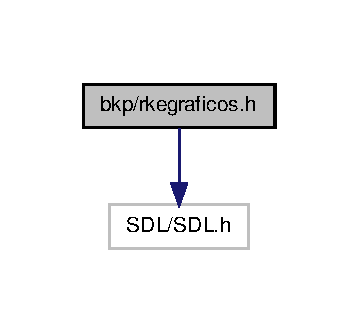
\includegraphics[width=172pt]{rkegraficos_8h__incl}
\end{center}
\end{figure}
Este grafo mostra quais arquivos estão direta ou indiretamente relacionados com este arquivo:
\nopagebreak
\begin{figure}[H]
\begin{center}
\leavevmode
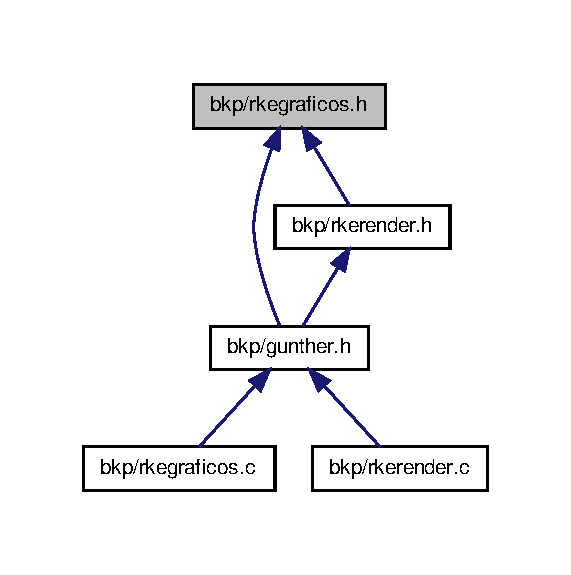
\includegraphics[width=274pt]{rkegraficos_8h__dep__incl}
\end{center}
\end{figure}
\subsection*{Definições e Macros}
\begin{DoxyCompactItemize}
\item 
\hypertarget{rkegraficos_8h_abb452686968e48b67397da5f97445f5b}{
\#define {\bfseries bool}~int}
\label{rkegraficos_8h_abb452686968e48b67397da5f97445f5b}

\item 
\hypertarget{rkegraficos_8h_a41f9c5fb8b08eb5dc3edce4dcb37fee7}{
\#define {\bfseries true}~1}
\label{rkegraficos_8h_a41f9c5fb8b08eb5dc3edce4dcb37fee7}

\item 
\hypertarget{rkegraficos_8h_a65e9886d74aaee76545e83dd09011727}{
\#define {\bfseries false}~0}
\label{rkegraficos_8h_a65e9886d74aaee76545e83dd09011727}

\item 
\hypertarget{rkegraficos_8h_a6d4fb88bc6adeca0366c73177965b146}{
\#define {\bfseries TAMMAX}~100}
\label{rkegraficos_8h_a6d4fb88bc6adeca0366c73177965b146}

\item 
\hypertarget{rkegraficos_8h_a0cfd5d3f47cf0b1f532c667efa58ec77}{
\#define {\bfseries IMAGEDIR}~\char`\"{}data/imagens/\char`\"{}}
\label{rkegraficos_8h_a0cfd5d3f47cf0b1f532c667efa58ec77}

\item 
\hypertarget{rkegraficos_8h_afb1f8b13a063e4f1e0b6c19ec6d07e97}{
\#define {\bfseries KEY\_\-VERMELHO}~0}
\label{rkegraficos_8h_afb1f8b13a063e4f1e0b6c19ec6d07e97}

\item 
\hypertarget{rkegraficos_8h_ab2b1135d6d5b6fc34dc751381487c3ce}{
\#define {\bfseries KEY\_\-VERDE}~0xFF}
\label{rkegraficos_8h_ab2b1135d6d5b6fc34dc751381487c3ce}

\item 
\hypertarget{rkegraficos_8h_a3b57b8b8e244e9f50bc24bffd15540fb}{
\#define {\bfseries KEY\_\-AZUL}~0xFF}
\label{rkegraficos_8h_a3b57b8b8e244e9f50bc24bffd15540fb}

\end{DoxyCompactItemize}
\subsection*{Funções}
\begin{DoxyCompactItemize}
\item 
SDL\_\-Surface $\ast$ \hyperlink{rkegraficos_8h_a53d0882910021c0b29435e2c04b4c341}{rke\_\-abre\_\-janela} (int largura, int altura)
\item 
void \hyperlink{rkegraficos_8h_a630239d2b9e61caeb0c1d6bdc8e78bab}{rke\_\-aplica\_\-tela} (SDL\_\-Surface $\ast$destino, SDL\_\-Surface $\ast$origem)
\item 
SDL\_\-Surface $\ast$ \hyperlink{rkegraficos_8h_ac56e3ff6e5a31f288b8f79b1b2deafb4}{rke\_\-carrega\_\-BMP} (char $\ast$arquivo)
\item 
void \hyperlink{rkegraficos_8h_aabf56f1febb197788ed7f0f0e08ddee1}{rke\_\-aplica\_\-clip\_\-duplo} (SDL\_\-Surface $\ast$destino, SDL\_\-Surface $\ast$origem, SDL\_\-Rect clip\mbox{[}$\,$\mbox{]}\mbox{[}2\mbox{]}, int selecao)
\item 
void \hyperlink{rkegraficos_8h_a950c17bba5cee25bbbce48eb76732d62}{rke\_\-carrega\_\-clip\_\-duplo} (char $\ast$arquivo, SDL\_\-Rect clip\mbox{[}$\,$\mbox{]}\mbox{[}2\mbox{]})
\item 
void \hyperlink{rkegraficos_8h_a904c2e2c797baab5f56609a7eb450e90}{rke\_\-libera\_\-tela} (SDL\_\-Surface $\ast$tela)
\item 
void \hyperlink{rkegraficos_8h_a93d1a1125deb9c4995b13208df7d5fa4}{rke\_\-aplica\_\-clip\_\-a\_\-mapa} (SDL\_\-Surface $\ast$destino, SDL\_\-Surface $\ast$origem, int mapa\_\-x, int mapa\_\-y, SDL\_\-Rect clip)
\end{DoxyCompactItemize}


\subsection{Descrição Detalhada}
Arquivo header da parte gráfica. \begin{DoxyAuthor}{Autor}
João da Silva, Marina Salles, Ricardo Macedo 
\end{DoxyAuthor}


\subsection{Funções}
\hypertarget{rkegraficos_8h_a53d0882910021c0b29435e2c04b4c341}{
\index{rkegraficos.h@{rkegraficos.h}!rke\_\-abre\_\-janela@{rke\_\-abre\_\-janela}}
\index{rke\_\-abre\_\-janela@{rke\_\-abre\_\-janela}!rkegraficos.h@{rkegraficos.h}}
\subsubsection[{rke\_\-abre\_\-janela}]{\setlength{\rightskip}{0pt plus 5cm}SDL\_\-Surface$\ast$ rke\_\-abre\_\-janela (
\begin{DoxyParamCaption}
\item[{int}]{largura, }
\item[{int}]{altura}
\end{DoxyParamCaption}
)}}
\label{rkegraficos_8h_a53d0882910021c0b29435e2c04b4c341}
Abre uma nova janela 
\begin{DoxyParams}{Parâmetros}
{\em largura} & Largura em pixels \\
\hline
{\em altura} & Altura em pixels \\
\hline
\end{DoxyParams}
\hypertarget{rkegraficos_8h_a93d1a1125deb9c4995b13208df7d5fa4}{
\index{rkegraficos.h@{rkegraficos.h}!rke\_\-aplica\_\-clip\_\-a\_\-mapa@{rke\_\-aplica\_\-clip\_\-a\_\-mapa}}
\index{rke\_\-aplica\_\-clip\_\-a\_\-mapa@{rke\_\-aplica\_\-clip\_\-a\_\-mapa}!rkegraficos.h@{rkegraficos.h}}
\subsubsection[{rke\_\-aplica\_\-clip\_\-a\_\-mapa}]{\setlength{\rightskip}{0pt plus 5cm}void rke\_\-aplica\_\-clip\_\-a\_\-mapa (
\begin{DoxyParamCaption}
\item[{SDL\_\-Surface $\ast$}]{destino, }
\item[{SDL\_\-Surface $\ast$}]{origem, }
\item[{int}]{mapa\_\-x, }
\item[{int}]{mapa\_\-y, }
\item[{SDL\_\-Rect}]{clip}
\end{DoxyParamCaption}
)}}
\label{rkegraficos_8h_a93d1a1125deb9c4995b13208df7d5fa4}
Aplica um retângulo a uma tela 
\begin{DoxyParams}{Parâmetros}
{\em destino} & A tela que receberá a imagem \\
\hline
{\em origem} & A tela de origem \\
\hline
{\em mapa\_\-x} & A posição X (em ladrilhos) no destino \\
\hline
{\em mapa\_\-y} & A posição Y (em ladrilhos) no destino \\
\hline
{\em clip} & O retângulo a ser aplicado \\
\hline
\end{DoxyParams}
\hypertarget{rkegraficos_8h_aabf56f1febb197788ed7f0f0e08ddee1}{
\index{rkegraficos.h@{rkegraficos.h}!rke\_\-aplica\_\-clip\_\-duplo@{rke\_\-aplica\_\-clip\_\-duplo}}
\index{rke\_\-aplica\_\-clip\_\-duplo@{rke\_\-aplica\_\-clip\_\-duplo}!rkegraficos.h@{rkegraficos.h}}
\subsubsection[{rke\_\-aplica\_\-clip\_\-duplo}]{\setlength{\rightskip}{0pt plus 5cm}void rke\_\-aplica\_\-clip\_\-duplo (
\begin{DoxyParamCaption}
\item[{SDL\_\-Surface $\ast$}]{destino, }
\item[{SDL\_\-Surface $\ast$}]{origem, }
\item[{SDL\_\-Rect}]{clip\mbox{[}$\,$\mbox{]}\mbox{[}2\mbox{]}, }
\item[{int}]{selecao}
\end{DoxyParamCaption}
)}}
\label{rkegraficos_8h_aabf56f1febb197788ed7f0f0e08ddee1}
Copia um retângulo em uma tela para um outro retângulo em outra tela 
\begin{DoxyParams}{Parâmetros}
{\em destino} & Tela de destino \\
\hline
{\em origem} & Tela de origem \\
\hline
{\em clip} & Vetor com os retângulos \\
\hline
{\em selecao} & Opção selecionada no menu \\
\hline
\end{DoxyParams}
\hypertarget{rkegraficos_8h_a630239d2b9e61caeb0c1d6bdc8e78bab}{
\index{rkegraficos.h@{rkegraficos.h}!rke\_\-aplica\_\-tela@{rke\_\-aplica\_\-tela}}
\index{rke\_\-aplica\_\-tela@{rke\_\-aplica\_\-tela}!rkegraficos.h@{rkegraficos.h}}
\subsubsection[{rke\_\-aplica\_\-tela}]{\setlength{\rightskip}{0pt plus 5cm}void rke\_\-aplica\_\-tela (
\begin{DoxyParamCaption}
\item[{SDL\_\-Surface $\ast$}]{destino, }
\item[{SDL\_\-Surface $\ast$}]{origem}
\end{DoxyParamCaption}
)}}
\label{rkegraficos_8h_a630239d2b9e61caeb0c1d6bdc8e78bab}
Aplica uma tela guardada em memória em outra 
\begin{DoxyParams}{Parâmetros}
{\em destino} & Tela de destino \\
\hline
{\em origem} & Tela de origem \\
\hline
\end{DoxyParams}
\hypertarget{rkegraficos_8h_ac56e3ff6e5a31f288b8f79b1b2deafb4}{
\index{rkegraficos.h@{rkegraficos.h}!rke\_\-carrega\_\-BMP@{rke\_\-carrega\_\-BMP}}
\index{rke\_\-carrega\_\-BMP@{rke\_\-carrega\_\-BMP}!rkegraficos.h@{rkegraficos.h}}
\subsubsection[{rke\_\-carrega\_\-BMP}]{\setlength{\rightskip}{0pt plus 5cm}SDL\_\-Surface$\ast$ rke\_\-carrega\_\-BMP (
\begin{DoxyParamCaption}
\item[{char $\ast$}]{arquivo}
\end{DoxyParamCaption}
)}}
\label{rkegraficos_8h_ac56e3ff6e5a31f288b8f79b1b2deafb4}
Carrega um arquivo Bitmap em uma tela 
\begin{DoxyParams}{Parâmetros}
{\em arquivo} & O nome do arquivo \\
\hline
\end{DoxyParams}
\hypertarget{rkegraficos_8h_a950c17bba5cee25bbbce48eb76732d62}{
\index{rkegraficos.h@{rkegraficos.h}!rke\_\-carrega\_\-clip\_\-duplo@{rke\_\-carrega\_\-clip\_\-duplo}}
\index{rke\_\-carrega\_\-clip\_\-duplo@{rke\_\-carrega\_\-clip\_\-duplo}!rkegraficos.h@{rkegraficos.h}}
\subsubsection[{rke\_\-carrega\_\-clip\_\-duplo}]{\setlength{\rightskip}{0pt plus 5cm}void rke\_\-carrega\_\-clip\_\-duplo (
\begin{DoxyParamCaption}
\item[{char $\ast$}]{arquivo, }
\item[{SDL\_\-Rect}]{clip\mbox{[}$\,$\mbox{]}\mbox{[}2\mbox{]}}
\end{DoxyParamCaption}
)}}
\label{rkegraficos_8h_a950c17bba5cee25bbbce48eb76732d62}
Carrega retângulos a partir de um arquivo 
\begin{DoxyParams}{Parâmetros}
{\em arquivo} & O arquivo a ser carregado \\
\hline
{\em clip} & O vetor de retângulos que conterá as informações \\
\hline
\end{DoxyParams}
\hypertarget{rkegraficos_8h_a904c2e2c797baab5f56609a7eb450e90}{
\index{rkegraficos.h@{rkegraficos.h}!rke\_\-libera\_\-tela@{rke\_\-libera\_\-tela}}
\index{rke\_\-libera\_\-tela@{rke\_\-libera\_\-tela}!rkegraficos.h@{rkegraficos.h}}
\subsubsection[{rke\_\-libera\_\-tela}]{\setlength{\rightskip}{0pt plus 5cm}void rke\_\-libera\_\-tela (
\begin{DoxyParamCaption}
\item[{SDL\_\-Surface $\ast$}]{tela}
\end{DoxyParamCaption}
)}}
\label{rkegraficos_8h_a904c2e2c797baab5f56609a7eb450e90}
Libera a memória de uma tela 
\begin{DoxyParams}{Parâmetros}
{\em tela} & A tela em questão \\
\hline
\end{DoxyParams}

\hypertarget{rkerender_8h}{
\section{Referência do Arquivo bkp/rkerender.h}
\label{rkerender_8h}\index{bkp/rkerender.h@{bkp/rkerender.h}}
}


Arquivo header do renderizador.  


{\ttfamily \#include \char`\"{}rkegraficos.h\char`\"{}}\par
Gráfico de dependência de inclusões para rkerender.h:
\nopagebreak
\begin{figure}[H]
\begin{center}
\leavevmode
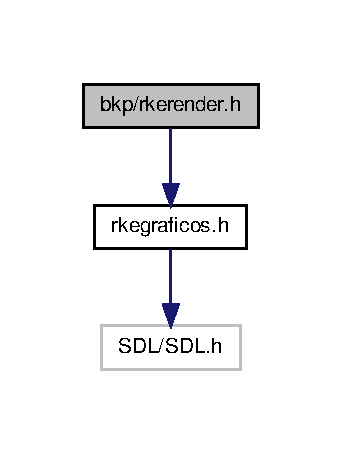
\includegraphics[width=164pt]{rkerender_8h__incl}
\end{center}
\end{figure}
Este grafo mostra quais arquivos estão direta ou indiretamente relacionados com este arquivo:
\nopagebreak
\begin{figure}[H]
\begin{center}
\leavevmode
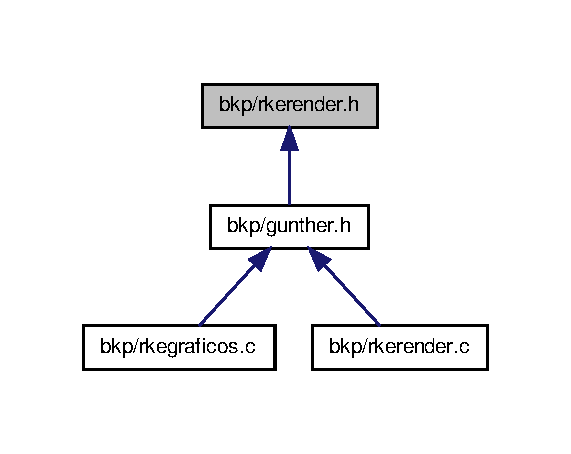
\includegraphics[width=274pt]{rkerender_8h__dep__incl}
\end{center}
\end{figure}
\subsection*{Estruturas de Dados}
\begin{DoxyCompactItemize}
\item 
struct \hyperlink{struct__ladrilho}{\_\-ladrilho}
\item 
struct \hyperlink{struct__tabuleiro}{\_\-tabuleiro}
\item 
struct \hyperlink{struct__objeto}{\_\-objeto}
\item 
struct \hyperlink{struct__jogador}{\_\-jogador}
\end{DoxyCompactItemize}
\subsection*{Definições e Macros}
\begin{DoxyCompactItemize}
\item 
\hypertarget{rkerender_8h_a0240ac851181b84ac374872dc5434ee4}{
\#define {\bfseries N}~0}
\label{rkerender_8h_a0240ac851181b84ac374872dc5434ee4}

\item 
\hypertarget{rkerender_8h_a5af9139e882aef6c820ae908589a40d6}{
\#define {\bfseries NE}~1}
\label{rkerender_8h_a5af9139e882aef6c820ae908589a40d6}

\item 
\hypertarget{rkerender_8h_a07484107e6d9fdf38b53edf631d6511d}{
\#define {\bfseries E}~2}
\label{rkerender_8h_a07484107e6d9fdf38b53edf631d6511d}

\item 
\hypertarget{rkerender_8h_a18bbe716f5be6adbd2150139244c0262}{
\#define {\bfseries SE}~3}
\label{rkerender_8h_a18bbe716f5be6adbd2150139244c0262}

\item 
\hypertarget{rkerender_8h_af933676109efed7ab34cea71d748a517}{
\#define {\bfseries S}~4}
\label{rkerender_8h_af933676109efed7ab34cea71d748a517}

\item 
\hypertarget{rkerender_8h_a02cc6d026fad97c4a8c84675a0619d03}{
\#define {\bfseries SO}~5}
\label{rkerender_8h_a02cc6d026fad97c4a8c84675a0619d03}

\item 
\hypertarget{rkerender_8h_a396fecfabe3105afc15a61c209f910f0}{
\#define {\bfseries O}~6}
\label{rkerender_8h_a396fecfabe3105afc15a61c209f910f0}

\item 
\hypertarget{rkerender_8h_a996bde01ecac342918f0a2c4e7ce7bd5}{
\#define {\bfseries NO}~7}
\label{rkerender_8h_a996bde01ecac342918f0a2c4e7ce7bd5}

\end{DoxyCompactItemize}
\subsection*{Definições de Tipos}
\begin{DoxyCompactItemize}
\item 
typedef struct \hyperlink{struct__ladrilho}{\_\-ladrilho} \hyperlink{rkerender_8h_a8be5d5879377ab21271dad6f3691f9fe}{Ladrilho}
\item 
typedef struct \hyperlink{struct__tabuleiro}{\_\-tabuleiro} \hyperlink{rkerender_8h_a0daefc5bc2fe00432f1dbe344d946d67}{Tabuleiro}
\item 
typedef struct \hyperlink{struct__objeto}{\_\-objeto} \hyperlink{rkerender_8h_a83af8ea0f645662f4b2b0d720cdf1748}{Objeto}
\item 
typedef struct \hyperlink{struct__jogador}{\_\-jogador} \hyperlink{rkerender_8h_a244c5487b0f580caedc3e744dfa296dc}{Jogador}
\end{DoxyCompactItemize}
\subsection*{Funções}
\begin{DoxyCompactItemize}
\item 
void \hyperlink{rkerender_8h_a95123d6fd00a9b48016c595c427eeb55}{rke\_\-render} (char $\ast$fase, char $\ast$imagens, char $\ast$img\_\-jogador, int larg, int alt, int largura\_\-ladrilho, int altura\_\-ladrilho)
\item 
void \hyperlink{rkerender_8h_a8dc5a9555b2b8a1e08c811a7a35469ea}{rke\_\-carrega\_\-terreno} (char $\ast$arquivo, \hyperlink{struct__ladrilho}{Ladrilho} terrenos\mbox{[}$\,$\mbox{]}, int larg\_\-ladrilho, int alt\_\-ladrilho)
\item 
void \hyperlink{rkerender_8h_af0f031a450b3be6ba5c5bc5b6d103653}{rke\_\-carrega\_\-objetos} (char $\ast$arquivo, \hyperlink{struct__objeto}{Objeto} objetos\mbox{[}$\,$\mbox{]}, int larg\_\-ladrilho, int alt\_\-ladrilho)
\item 
void \hyperlink{rkerender_8h_aaa263ecd9eccd396516779b7ef6710f6}{rke\_\-carrega\_\-fase} (char $\ast$arquivo, \hyperlink{struct__tabuleiro}{Tabuleiro} $\ast$tabuleiro, int $\ast$jogador\_\-x, int $\ast$jogador\_\-y)
\item 
void \hyperlink{rkerender_8h_a367aed7c3de5f557a25d934be4aee8a4}{rke\_\-carrega\_\-jogador} (\hyperlink{struct__jogador}{Jogador} $\ast$jogador, int larg\_\-ladrilho, int alt\_\-ladrilho)
\item 
void \hyperlink{rkerender_8h_a4fb57e2863d45d122b3cfa8b70a78aa9}{rke\_\-move\_\-jogador} (\hyperlink{struct__jogador}{Jogador} $\ast$jogador, \hyperlink{struct__tabuleiro}{Tabuleiro} tabuleiro, \hyperlink{struct__ladrilho}{Ladrilho} $\ast$terrenos, \hyperlink{struct__objeto}{Objeto} $\ast$objetos, int delta\_\-x, int delta\_\-y)
\end{DoxyCompactItemize}
\subsection*{Variáveis}
\begin{DoxyCompactItemize}
\item 
\hypertarget{rkerender_8h_aa6f5f4c21bc998af7d9449a286c7f4d7}{
$<$$<$$<$$<$$<$$<$$<$ HEAD:include/rkerender.hvoidrke\_\-jogador\_\-atira(\hyperlink{struct__jogador}{Jogador} $\ast$jogador, Tabuleirotabuleiro, \hyperlink{struct__ladrilho}{Ladrilho} $\ast$terrenos, \hyperlink{struct__objeto}{Objeto} $\ast$objetos, intbomba);=======voidrke\_\-jogador\_\-atira(\hyperlink{struct__jogador}{Jogador} $\ast$jogador, Tabuleirotabuleiro, \hyperlink{struct__ladrilho}{Ladrilho} $\ast$terrenos, \hyperlink{struct__objeto}{Objeto} $\ast$objetos);$>$$>$$>$$>$$>$ {\bfseries towers\_\-bombs} )}
\label{rkerender_8h_aa6f5f4c21bc998af7d9449a286c7f4d7}

\item 
\hypertarget{rkerender_8h_a76157e56d976652d4a91333e12277f13}{
$<$$<$$<$$<$$<$$<$$<$ HEAD:include/rkerender.hvoidrke\_\-jogador\_\-atira(\hyperlink{struct__jogador}{Jogador} $\ast$jogador, Tabuleirotabuleiro, \hyperlink{struct__ladrilho}{Ladrilho} $\ast$terrenos, \hyperlink{struct__objeto}{Objeto} $\ast$objetos, intbomba);=======voidrke\_\-jogador\_\-atira(\hyperlink{struct__jogador}{Jogador} $\ast$jogador, Tabuleirotabuleiro, \hyperlink{struct__ladrilho}{Ladrilho} $\ast$terrenos, \hyperlink{struct__objeto}{Objeto} $\ast$objetos);$>$$>$$>$$>$$>$$>$ Tabuleir {\bfseries tabuleiro} )}
\label{rkerender_8h_a76157e56d976652d4a91333e12277f13}

\item 
\hypertarget{rkerender_8h_a7bc9819464506dedf668039b7759f5fb}{
$<$$<$$<$$<$$<$$<$$<$ HEAD:include/rkerender.hvoidrke\_\-jogador\_\-atira(\hyperlink{struct__jogador}{Jogador} $\ast$jogador, Tabuleirotabuleiro, \hyperlink{struct__ladrilho}{Ladrilho} $\ast$terrenos, \hyperlink{struct__objeto}{Objeto} $\ast$objetos, intbomba);=======voidrke\_\-jogador\_\-atira(\hyperlink{struct__jogador}{Jogador} $\ast$jogador, Tabuleirotabuleiro, \hyperlink{struct__ladrilho}{Ladrilho} $\ast$terrenos, \hyperlink{struct__objeto}{Objeto} $\ast$objetos);$>$$>$$>$$>$$>$$>$ \hyperlink{struct__tabuleiro}{Tabuleiro} \hyperlink{struct__ladrilho}{Ladrilho} {\bfseries terrenos} )}
\label{rkerender_8h_a7bc9819464506dedf668039b7759f5fb}

\item 
\hypertarget{rkerender_8h_a815e186b3e2b277fdc172f305cc5fedf}{
$<$$<$$<$$<$$<$$<$$<$ HEAD:include/rkerender.hvoidrke\_\-jogador\_\-atira(\hyperlink{struct__jogador}{Jogador} $\ast$jogador, Tabuleirotabuleiro, \hyperlink{struct__ladrilho}{Ladrilho} $\ast$terrenos, \hyperlink{struct__objeto}{Objeto} $\ast$objetos, intbomba);=======voidrke\_\-jogador\_\-atira(\hyperlink{struct__jogador}{Jogador} $\ast$jogador, Tabuleirotabuleiro, \hyperlink{struct__ladrilho}{Ladrilho} $\ast$terrenos, \hyperlink{struct__objeto}{Objeto} $\ast$objetos);$>$$>$$>$$>$$>$$>$ \hyperlink{struct__tabuleiro}{Tabuleiro} \hyperlink{struct__ladrilho}{Ladrilho} \hyperlink{struct__objeto}{Objeto} {\bfseries objetos} )}
\label{rkerender_8h_a815e186b3e2b277fdc172f305cc5fedf}

\end{DoxyCompactItemize}


\subsection{Descrição Detalhada}
Arquivo header do renderizador. \begin{DoxyAuthor}{Autor}
João da Silva, Marina Salles, Ricardo Macedo 
\end{DoxyAuthor}


\subsection{Definições dos tipos}
\hypertarget{rkerender_8h_a244c5487b0f580caedc3e744dfa296dc}{
\index{rkerender.h@{rkerender.h}!Jogador@{Jogador}}
\index{Jogador@{Jogador}!rkerender.h@{rkerender.h}}
\subsubsection[{Jogador}]{\setlength{\rightskip}{0pt plus 5cm}typedef struct {\bf \_\-jogador}  {\bf Jogador}}}
\label{rkerender_8h_a244c5487b0f580caedc3e744dfa296dc}
Struct Jogador 
\begin{DoxyParams}{Parâmetros}
{\em retangulo} & Vetor com os 8 retângulos das visões do jogador \\
\hline
{\em x} & Posição x do jogador \\
\hline
{\em y} & Posição y do jogador \\
\hline
{\em direcao} & Direção que o jogador está olhando \\
\hline
{\em hp} & Quantidade de hp do jogador \\
\hline
\end{DoxyParams}
\hypertarget{rkerender_8h_a8be5d5879377ab21271dad6f3691f9fe}{
\index{rkerender.h@{rkerender.h}!Ladrilho@{Ladrilho}}
\index{Ladrilho@{Ladrilho}!rkerender.h@{rkerender.h}}
\subsubsection[{Ladrilho}]{\setlength{\rightskip}{0pt plus 5cm}typedef struct {\bf \_\-ladrilho}  {\bf Ladrilho}}}
\label{rkerender_8h_a8be5d5879377ab21271dad6f3691f9fe}
Struct Ladrilho 
\begin{DoxyParams}{Parâmetros}
{\em retangulo} & Retângulo do ladrilho no clipboard \\
\hline
{\em passavel} & Indica se o jogador pode andar em cima do ladrilho \\
\hline
\end{DoxyParams}
\hypertarget{rkerender_8h_a83af8ea0f645662f4b2b0d720cdf1748}{
\index{rkerender.h@{rkerender.h}!Objeto@{Objeto}}
\index{Objeto@{Objeto}!rkerender.h@{rkerender.h}}
\subsubsection[{Objeto}]{\setlength{\rightskip}{0pt plus 5cm}typedef struct {\bf \_\-objeto}  {\bf Objeto}}}
\label{rkerender_8h_a83af8ea0f645662f4b2b0d720cdf1748}
Struct Objeto 
\begin{DoxyParams}{Parâmetros}
{\em retangulo} & Retângulo da imagem do objeto no clipboard \\
\hline
{\em hp} & Quantidade de hp do objeto \\
\hline
{\em attack} & Tipo de ataque do objeto \\
\hline
{\em bonus} & Tipo de bonus do objeto \\
\hline
\end{DoxyParams}
\hypertarget{rkerender_8h_a0daefc5bc2fe00432f1dbe344d946d67}{
\index{rkerender.h@{rkerender.h}!Tabuleiro@{Tabuleiro}}
\index{Tabuleiro@{Tabuleiro}!rkerender.h@{rkerender.h}}
\subsubsection[{Tabuleiro}]{\setlength{\rightskip}{0pt plus 5cm}typedef struct {\bf \_\-tabuleiro}  {\bf Tabuleiro}}}
\label{rkerender_8h_a0daefc5bc2fe00432f1dbe344d946d67}
Struct Tabuleiro 
\begin{DoxyParams}{Parâmetros}
{\em terreno} & Matriz que armazena como o terreno é construído \\
\hline
{\em objetos} & Matriz que armazena a localização dos objetos \\
\hline
\end{DoxyParams}


\subsection{Funções}
\hypertarget{rkerender_8h_aaa263ecd9eccd396516779b7ef6710f6}{
\index{rkerender.h@{rkerender.h}!rke\_\-carrega\_\-fase@{rke\_\-carrega\_\-fase}}
\index{rke\_\-carrega\_\-fase@{rke\_\-carrega\_\-fase}!rkerender.h@{rkerender.h}}
\subsubsection[{rke\_\-carrega\_\-fase}]{\setlength{\rightskip}{0pt plus 5cm}void rke\_\-carrega\_\-fase (
\begin{DoxyParamCaption}
\item[{char $\ast$}]{arquivo, }
\item[{{\bf Tabuleiro} $\ast$}]{tabuleiro, }
\item[{int $\ast$}]{jogador\_\-x, }
\item[{int $\ast$}]{jogador\_\-y}
\end{DoxyParamCaption}
)}}
\label{rkerender_8h_aaa263ecd9eccd396516779b7ef6710f6}
Carrega as informações do tabuleiro da fase 
\begin{DoxyParams}{Parâmetros}
{\em arquivo} & O arquivo com as informações \\
\hline
{\em tabuleiro} & O lugar para armazenar as informações \\
\hline
{\em jogador\_\-x} & Argumento que devolve a posição X do jogador \\
\hline
{\em jogador\_\-y} & Argumento que devolve a posição Y do jogador \\
\hline
\end{DoxyParams}
\hypertarget{rkerender_8h_a367aed7c3de5f557a25d934be4aee8a4}{
\index{rkerender.h@{rkerender.h}!rke\_\-carrega\_\-jogador@{rke\_\-carrega\_\-jogador}}
\index{rke\_\-carrega\_\-jogador@{rke\_\-carrega\_\-jogador}!rkerender.h@{rkerender.h}}
\subsubsection[{rke\_\-carrega\_\-jogador}]{\setlength{\rightskip}{0pt plus 5cm}void rke\_\-carrega\_\-jogador (
\begin{DoxyParamCaption}
\item[{{\bf Jogador} $\ast$}]{jogador, }
\item[{int}]{larg\_\-ladrilho, }
\item[{int}]{alt\_\-ladrilho}
\end{DoxyParamCaption}
)}}
\label{rkerender_8h_a367aed7c3de5f557a25d934be4aee8a4}
Carrega os retângulos da imagem do jogador 
\begin{DoxyParams}{Parâmetros}
{\em O} & lugar para armazenar as informações \\
\hline
{\em Largura} & em pixels do ladrilho \\
\hline
{\em Altura} & em pixels do ladrilho \\
\hline
\end{DoxyParams}
\hypertarget{rkerender_8h_af0f031a450b3be6ba5c5bc5b6d103653}{
\index{rkerender.h@{rkerender.h}!rke\_\-carrega\_\-objetos@{rke\_\-carrega\_\-objetos}}
\index{rke\_\-carrega\_\-objetos@{rke\_\-carrega\_\-objetos}!rkerender.h@{rkerender.h}}
\subsubsection[{rke\_\-carrega\_\-objetos}]{\setlength{\rightskip}{0pt plus 5cm}void rke\_\-carrega\_\-objetos (
\begin{DoxyParamCaption}
\item[{char $\ast$}]{arquivo, }
\item[{{\bf Objeto}}]{objetos\mbox{[}$\,$\mbox{]}, }
\item[{int}]{larg\_\-ladrilho, }
\item[{int}]{alt\_\-ladrilho}
\end{DoxyParamCaption}
)}}
\label{rkerender_8h_af0f031a450b3be6ba5c5bc5b6d103653}
Carrega as informações dos objetos de um arquivo 
\begin{DoxyParams}{Parâmetros}
{\em arquivo} & O arquivo com as informações \\
\hline
{\em objetos} & O lugar para armazenar as informações \\
\hline
{\em larg\_\-ladrilho} & Largura em pixels do ladrilho \\
\hline
{\em alt\_\-ladrilho} & Altura em pixels do ladrilho \\
\hline
\end{DoxyParams}
\hypertarget{rkerender_8h_a8dc5a9555b2b8a1e08c811a7a35469ea}{
\index{rkerender.h@{rkerender.h}!rke\_\-carrega\_\-terreno@{rke\_\-carrega\_\-terreno}}
\index{rke\_\-carrega\_\-terreno@{rke\_\-carrega\_\-terreno}!rkerender.h@{rkerender.h}}
\subsubsection[{rke\_\-carrega\_\-terreno}]{\setlength{\rightskip}{0pt plus 5cm}void rke\_\-carrega\_\-terreno (
\begin{DoxyParamCaption}
\item[{char $\ast$}]{arquivo, }
\item[{{\bf Ladrilho}}]{terrenos\mbox{[}$\,$\mbox{]}, }
\item[{int}]{larg\_\-ladrilho, }
\item[{int}]{alt\_\-ladrilho}
\end{DoxyParamCaption}
)}}
\label{rkerender_8h_a8dc5a9555b2b8a1e08c811a7a35469ea}
Carrega as informações dos elementos de terreno de um arquivo 
\begin{DoxyParams}{Parâmetros}
{\em arquivo} & O arquivo com as informações \\
\hline
{\em terrenos} & O lugar para armazenar as informações \\
\hline
{\em larg\_\-ladrilho} & Largura em pixels do ladrilho \\
\hline
{\em alt\_\-ladrilho} & Altura em pixels do ladrilho \\
\hline
\end{DoxyParams}
\hypertarget{rkerender_8h_a4fb57e2863d45d122b3cfa8b70a78aa9}{
\index{rkerender.h@{rkerender.h}!rke\_\-move\_\-jogador@{rke\_\-move\_\-jogador}}
\index{rke\_\-move\_\-jogador@{rke\_\-move\_\-jogador}!rkerender.h@{rkerender.h}}
\subsubsection[{rke\_\-move\_\-jogador}]{\setlength{\rightskip}{0pt plus 5cm}void rke\_\-move\_\-jogador (
\begin{DoxyParamCaption}
\item[{{\bf Jogador} $\ast$}]{jogador, }
\item[{{\bf Tabuleiro}}]{tabuleiro, }
\item[{{\bf Ladrilho} $\ast$}]{terrenos, }
\item[{{\bf Objeto} $\ast$}]{objetos, }
\item[{int}]{delta\_\-x, }
\item[{int}]{delta\_\-y}
\end{DoxyParamCaption}
)}}
\label{rkerender_8h_a4fb57e2863d45d122b3cfa8b70a78aa9}
Função de movimentação do jogador. 
\begin{DoxyParams}{Parâmetros}
{\em jogador} & Informações do jogador \\
\hline
{\em tabuleiro} & Informações do tabuleiro \\
\hline
{\em terrenos} & Informações dos elementos de terreno \\
\hline
{\em objetos} & Informações dos objetos \\
\hline
{\em delta\_\-x} & Movimentação no eixo X \\
\hline
{\em delta\_\-y} & Movimentação no eixo Y \\
\hline
\end{DoxyParams}
\hypertarget{rkerender_8h_a95123d6fd00a9b48016c595c427eeb55}{
\index{rkerender.h@{rkerender.h}!rke\_\-render@{rke\_\-render}}
\index{rke\_\-render@{rke\_\-render}!rkerender.h@{rkerender.h}}
\subsubsection[{rke\_\-render}]{\setlength{\rightskip}{0pt plus 5cm}void rke\_\-render (
\begin{DoxyParamCaption}
\item[{char $\ast$}]{fase, }
\item[{char $\ast$}]{imagens, }
\item[{char $\ast$}]{img\_\-jogador, }
\item[{int}]{largura, }
\item[{int}]{altura, }
\item[{int}]{larg\_\-ladrilho, }
\item[{int}]{alt\_\-ladrilho}
\end{DoxyParamCaption}
)}}
\label{rkerender_8h_a95123d6fd00a9b48016c595c427eeb55}
Função principal do renderizador de fases 
\begin{DoxyParams}{Parâmetros}
{\em fase} & Arquivo de fase \\
\hline
{\em imagens} & Arquivo clipboard com as imagens para terreno e objetos \\
\hline
{\em img\_\-jogador} & Arquivo clipboard com as imagens do jogador \\
\hline
{\em largura} & Largura em ladrilhos da tela \\
\hline
{\em altura} & Altura em ladrilhos da tela \\
\hline
{\em larg\_\-ladrilho} & Largura em pixels do ladrilho \\
\hline
{\em alt\_\-ladrilho} & Altura em pixels do ladrilho \\
\hline
\end{DoxyParams}

\hypertarget{rketypes_8h}{
\section{Referência do Arquivo bkp/rketypes.h}
\label{rketypes_8h}\index{bkp/rketypes.h@{bkp/rketypes.h}}
}


Arquivo header de tipos e defines do Red Knife Engine.  


Este grafo mostra quais arquivos estão direta ou indiretamente relacionados com este arquivo:
\nopagebreak
\begin{figure}[H]
\begin{center}
\leavevmode
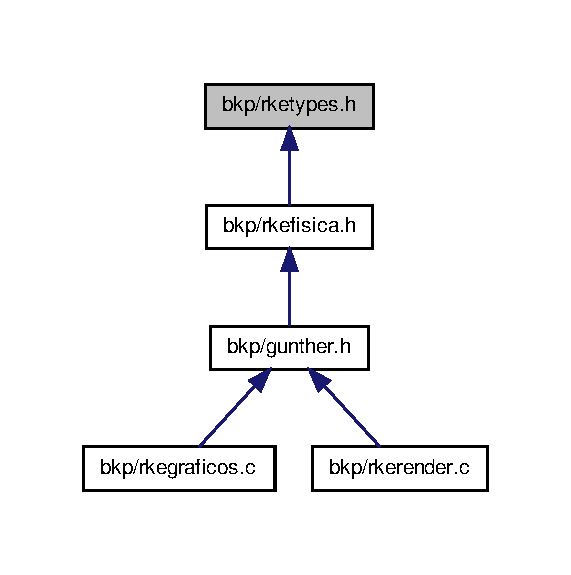
\includegraphics[width=274pt]{rketypes_8h__dep__incl}
\end{center}
\end{figure}
\subsection*{Estruturas de Dados}
\begin{DoxyCompactItemize}
\item 
struct \hyperlink{structstruct__vetor}{struct\_\-vetor}
\item 
struct \hyperlink{structstruct__objeto}{struct\_\-objeto}
\end{DoxyCompactItemize}
\subsection*{Definições e Macros}
\begin{DoxyCompactItemize}
\item 
\hypertarget{rketypes_8h_a446118036aeca9a42bc2d451ab80b8b7}{
\#define {\bfseries BARCOID}~-\/1}
\label{rketypes_8h_a446118036aeca9a42bc2d451ab80b8b7}

\item 
\hypertarget{rketypes_8h_a58883c467f961c4b1f998d575f943890}{
\#define {\bfseries ESTATICO}~-\/1.0}
\label{rketypes_8h_a58883c467f961c4b1f998d575f943890}

\end{DoxyCompactItemize}
\subsection*{Definições de Tipos}
\begin{DoxyCompactItemize}
\item 
typedef struct \hyperlink{structstruct__vetor}{struct\_\-vetor} \hyperlink{rketypes_8h_a27896866572b2a12760a22ea2654ed47}{vetor}
\item 
typedef struct \hyperlink{structstruct__objeto}{struct\_\-objeto} \hyperlink{rketypes_8h_a216693704a51093135790527237245ec}{objeto}
\end{DoxyCompactItemize}


\subsection{Descrição Detalhada}
Arquivo header de tipos e defines do Red Knife Engine. \begin{DoxyAuthor}{Autor}
João da Silva, Marina Salles, Ricardo Macedo 
\end{DoxyAuthor}


\subsection{Definições dos tipos}
\hypertarget{rketypes_8h_a216693704a51093135790527237245ec}{
\index{rketypes.h@{rketypes.h}!objeto@{objeto}}
\index{objeto@{objeto}!rketypes.h@{rketypes.h}}
\subsubsection[{objeto}]{\setlength{\rightskip}{0pt plus 5cm}typedef struct {\bf struct\_\-objeto}  {\bf objeto}}}
\label{rketypes_8h_a216693704a51093135790527237245ec}
Struct objeto 
\begin{DoxyParams}{Parâmetros}
{\em id} & Identificador único \\
\hline
{\em x} & Componente x \\
\hline
{\em y} & Componente y \\
\hline
{\em v\_\-x} & Componente x da velocidade do objeto \\
\hline
{\em v\_\-y} & Componente y da velocidade do objeto \\
\hline
{\em massa} & Massa do objeto \\
\hline
{\em tempo} & Tempo de vida do objeto \\
\hline
\end{DoxyParams}
\hypertarget{rketypes_8h_a27896866572b2a12760a22ea2654ed47}{
\index{rketypes.h@{rketypes.h}!vetor@{vetor}}
\index{vetor@{vetor}!rketypes.h@{rketypes.h}}
\subsubsection[{vetor}]{\setlength{\rightskip}{0pt plus 5cm}typedef struct {\bf struct\_\-vetor}  {\bf vetor}}}
\label{rketypes_8h_a27896866572b2a12760a22ea2654ed47}
Struct vetor 
\begin{DoxyParams}{Parâmetros}
{\em x} & Componente x \\
\hline
{\em y} & Componente y \\
\hline
\end{DoxyParams}

\hypertarget{main_8c}{\section{src/main.c File Reference}
\label{main_8c}\index{src/main.\-c@{src/main.\-c}}
}


Este é o arquivo que implementa as funções descritas na \hyperlink{fisica_8c}{fisica.\-c}. Aqui, carrega-\/se um arquivo texto com as condições iniciais e escreve um arquivo \char`\"{}saida.\-out\char`\"{} com as informações após as iterações.  


{\ttfamily \#include $<$stdio.\-h$>$}\\*
{\ttfamily \#include $<$stdlib.\-h$>$}\\*
{\ttfamily \#include $<$string.\-h$>$}\\*
{\ttfamily \#include \char`\"{}../include/rketypes.\-h\char`\"{}}\\*
{\ttfamily \#include \char`\"{}../include/rkefisica.\-h\char`\"{}}\\*
Include dependency graph for main.\-c\-:
\subsection*{Functions}
\begin{DoxyCompactItemize}
\item 
\hypertarget{main_8c_a0ddf1224851353fc92bfbff6f499fa97}{int {\bfseries main} (int argc, char $\ast$argv\mbox{[}$\,$\mbox{]})}\label{main_8c_a0ddf1224851353fc92bfbff6f499fa97}

\end{DoxyCompactItemize}


\subsection{Detailed Description}
Este é o arquivo que implementa as funções descritas na \hyperlink{fisica_8c}{fisica.\-c}. Aqui, carrega-\/se um arquivo texto com as condições iniciais e escreve um arquivo \char`\"{}saida.\-out\char`\"{} com as informações após as iterações. \begin{DoxyAuthor}{Author}
João da Silva, Marina Salles, Ricardo Macedo 
\end{DoxyAuthor}

\hypertarget{menu_8c}{
\section{Referência do Arquivo menu.c}
\label{menu_8c}\index{menu.c@{menu.c}}
}


Implementação do menu principal.  


{\ttfamily \#include \char`\"{}headers.h\char`\"{}}\par
Gráfico de dependência de inclusões para menu.c:\nopagebreak
\begin{figure}[H]
\begin{center}
\leavevmode
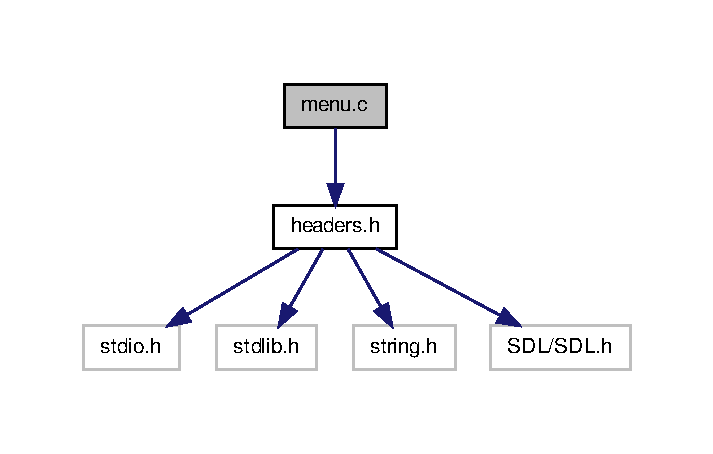
\includegraphics[width=342pt]{menu_8c__incl}
\end{center}
\end{figure}
\subsection*{Funções}
\begin{DoxyCompactItemize}
\item 
void \hyperlink{menu_8c_a54ce253826e283991f35d6a97d346a46}{gunther\_\-menu} (SDL\_\-Surface $\ast$screen)
\item 
int \hyperlink{menu_8c_a79fb862d32102adb3afd6c4850efa80f}{title} (SDL\_\-Surface $\ast$screen)
\item 
int \hyperlink{menu_8c_a4f64a22b2d93a0825625d69dec8b5524}{manual} (SDL\_\-Surface $\ast$screen, int mode)
\item 
\hypertarget{menu_8c_a7d1a4254bb9ad756b0528b4c95be9443}{
int {\bfseries options} (SDL\_\-Surface $\ast$screen)}
\label{menu_8c_a7d1a4254bb9ad756b0528b4c95be9443}

\item 
\hypertarget{menu_8c_af26f6b5c02e28bd5037ef7ee6dc2e2cf}{
int {\bfseries intro} (SDL\_\-Surface $\ast$screen)}
\label{menu_8c_af26f6b5c02e28bd5037ef7ee6dc2e2cf}

\item 
\hypertarget{menu_8c_a10e82c49851064a9aae3397425f5b936}{
int {\bfseries credits} (SDL\_\-Surface $\ast$screen)}
\label{menu_8c_a10e82c49851064a9aae3397425f5b936}

\end{DoxyCompactItemize}


\subsection{Descrição Detalhada}
Implementação do menu principal. \begin{DoxyAuthor}{Autor}
João da Silva, Marina Salles, Ricardo Macedo 
\end{DoxyAuthor}


\subsection{Funções}
\hypertarget{menu_8c_a54ce253826e283991f35d6a97d346a46}{
\index{menu.c@{menu.c}!gunther\_\-menu@{gunther\_\-menu}}
\index{gunther\_\-menu@{gunther\_\-menu}!menu.c@{menu.c}}
\subsubsection[{gunther\_\-menu}]{\setlength{\rightskip}{0pt plus 5cm}void gunther\_\-menu (
\begin{DoxyParamCaption}
\item[{SDL\_\-Surface $\ast$}]{screen}
\end{DoxyParamCaption}
)}}
\label{menu_8c_a54ce253826e283991f35d6a97d346a46}
Renderiza o menu baseado na seleção 
\begin{DoxyParams}{Parâmetros}
{\em tela} & Tela onde o menu será renderizado \\
\hline
\end{DoxyParams}
\hypertarget{menu_8c_a4f64a22b2d93a0825625d69dec8b5524}{
\index{menu.c@{menu.c}!manual@{manual}}
\index{manual@{manual}!menu.c@{menu.c}}
\subsubsection[{manual}]{\setlength{\rightskip}{0pt plus 5cm}int manual (
\begin{DoxyParamCaption}
\item[{SDL\_\-Surface $\ast$}]{screen, }
\item[{int}]{mode}
\end{DoxyParamCaption}
)}}
\label{menu_8c_a4f64a22b2d93a0825625d69dec8b5524}
Seção \char`\"{}Manual\char`\"{} do menu 
\begin{DoxyParams}{Parâmetros}
{\em tela} & Tela onde a seção será renderizada \\
\hline
\end{DoxyParams}
\hypertarget{menu_8c_a79fb862d32102adb3afd6c4850efa80f}{
\index{menu.c@{menu.c}!title@{title}}
\index{title@{title}!menu.c@{menu.c}}
\subsubsection[{title}]{\setlength{\rightskip}{0pt plus 5cm}int title (
\begin{DoxyParamCaption}
\item[{SDL\_\-Surface $\ast$}]{screen}
\end{DoxyParamCaption}
)}}
\label{menu_8c_a79fb862d32102adb3afd6c4850efa80f}
Menu principal 
\begin{DoxyParams}{Parâmetros}
{\em tela} & Tela onde o menu será renderizado \\
\hline
\end{DoxyParams}

\hypertarget{rkegraficos_8c}{
\section{Referência do Arquivo bkp/rkegraficos.c}
\label{rkegraficos_8c}\index{bkp/rkegraficos.c@{bkp/rkegraficos.c}}
}


Utilitários gráficos.  


{\ttfamily \#include \char`\"{}gunther.h\char`\"{}}\par
Gráfico de dependência de inclusões para rkegraficos.c:
\nopagebreak
\begin{figure}[H]
\begin{center}
\leavevmode
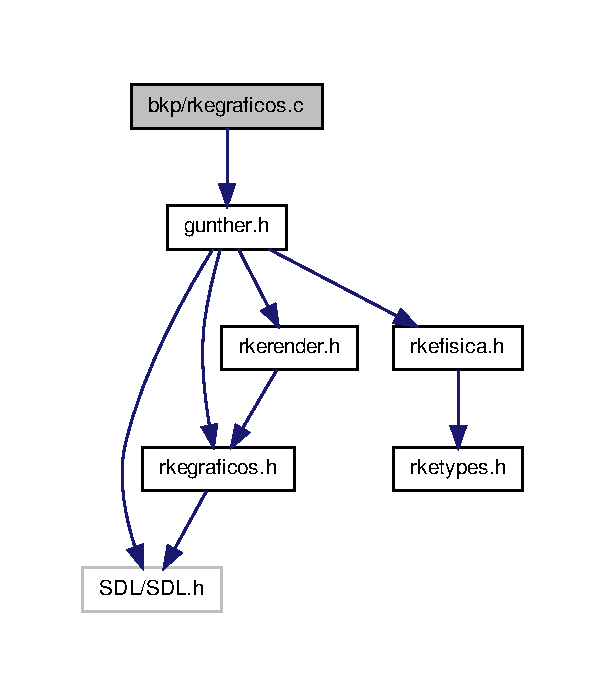
\includegraphics[width=291pt]{rkegraficos_8c__incl}
\end{center}
\end{figure}
\subsection*{Funções}
\begin{DoxyCompactItemize}
\item 
SDL\_\-Surface $\ast$ \hyperlink{rkegraficos_8c_a53d0882910021c0b29435e2c04b4c341}{rke\_\-abre\_\-janela} (int largura, int altura)
\item 
void \hyperlink{rkegraficos_8c_a630239d2b9e61caeb0c1d6bdc8e78bab}{rke\_\-aplica\_\-tela} (SDL\_\-Surface $\ast$destino, SDL\_\-Surface $\ast$origem)
\item 
SDL\_\-Surface $\ast$ \hyperlink{rkegraficos_8c_ac56e3ff6e5a31f288b8f79b1b2deafb4}{rke\_\-carrega\_\-BMP} (char $\ast$arquivo)
\item 
void \hyperlink{rkegraficos_8c_aabf56f1febb197788ed7f0f0e08ddee1}{rke\_\-aplica\_\-clip\_\-duplo} (SDL\_\-Surface $\ast$destino, SDL\_\-Surface $\ast$origem, SDL\_\-Rect clip\mbox{[}$\,$\mbox{]}\mbox{[}2\mbox{]}, int selecao)
\item 
void \hyperlink{rkegraficos_8c_a950c17bba5cee25bbbce48eb76732d62}{rke\_\-carrega\_\-clip\_\-duplo} (char $\ast$arquivo, SDL\_\-Rect clip\mbox{[}$\,$\mbox{]}\mbox{[}2\mbox{]})
\item 
void \hyperlink{rkegraficos_8c_a904c2e2c797baab5f56609a7eb450e90}{rke\_\-libera\_\-tela} (SDL\_\-Surface $\ast$tela)
\item 
void \hyperlink{rkegraficos_8c_a93d1a1125deb9c4995b13208df7d5fa4}{rke\_\-aplica\_\-clip\_\-a\_\-mapa} (SDL\_\-Surface $\ast$destino, SDL\_\-Surface $\ast$origem, int mapa\_\-x, int mapa\_\-y, SDL\_\-Rect clip)
\end{DoxyCompactItemize}


\subsection{Descrição Detalhada}
Utilitários gráficos. \begin{DoxyAuthor}{Autor}
João da Silva, Marina Salles, Ricardo Macedo 
\end{DoxyAuthor}


\subsection{Funções}
\hypertarget{rkegraficos_8c_a53d0882910021c0b29435e2c04b4c341}{
\index{rkegraficos.c@{rkegraficos.c}!rke\_\-abre\_\-janela@{rke\_\-abre\_\-janela}}
\index{rke\_\-abre\_\-janela@{rke\_\-abre\_\-janela}!rkegraficos.c@{rkegraficos.c}}
\subsubsection[{rke\_\-abre\_\-janela}]{\setlength{\rightskip}{0pt plus 5cm}SDL\_\-Surface$\ast$ rke\_\-abre\_\-janela (
\begin{DoxyParamCaption}
\item[{int}]{largura, }
\item[{int}]{altura}
\end{DoxyParamCaption}
)}}
\label{rkegraficos_8c_a53d0882910021c0b29435e2c04b4c341}
Abre uma nova janela 
\begin{DoxyParams}{Parâmetros}
{\em largura} & Largura em pixels \\
\hline
{\em altura} & Altura em pixels \\
\hline
\end{DoxyParams}
\hypertarget{rkegraficos_8c_a93d1a1125deb9c4995b13208df7d5fa4}{
\index{rkegraficos.c@{rkegraficos.c}!rke\_\-aplica\_\-clip\_\-a\_\-mapa@{rke\_\-aplica\_\-clip\_\-a\_\-mapa}}
\index{rke\_\-aplica\_\-clip\_\-a\_\-mapa@{rke\_\-aplica\_\-clip\_\-a\_\-mapa}!rkegraficos.c@{rkegraficos.c}}
\subsubsection[{rke\_\-aplica\_\-clip\_\-a\_\-mapa}]{\setlength{\rightskip}{0pt plus 5cm}void rke\_\-aplica\_\-clip\_\-a\_\-mapa (
\begin{DoxyParamCaption}
\item[{SDL\_\-Surface $\ast$}]{destino, }
\item[{SDL\_\-Surface $\ast$}]{origem, }
\item[{int}]{mapa\_\-x, }
\item[{int}]{mapa\_\-y, }
\item[{SDL\_\-Rect}]{clip}
\end{DoxyParamCaption}
)}}
\label{rkegraficos_8c_a93d1a1125deb9c4995b13208df7d5fa4}
Aplica um retângulo a uma tela 
\begin{DoxyParams}{Parâmetros}
{\em destino} & A tela que receberá a imagem \\
\hline
{\em origem} & A tela de origem \\
\hline
{\em mapa\_\-x} & A posição X (em ladrilhos) no destino \\
\hline
{\em mapa\_\-y} & A posição Y (em ladrilhos) no destino \\
\hline
{\em clip} & O retângulo a ser aplicado \\
\hline
\end{DoxyParams}
\hypertarget{rkegraficos_8c_aabf56f1febb197788ed7f0f0e08ddee1}{
\index{rkegraficos.c@{rkegraficos.c}!rke\_\-aplica\_\-clip\_\-duplo@{rke\_\-aplica\_\-clip\_\-duplo}}
\index{rke\_\-aplica\_\-clip\_\-duplo@{rke\_\-aplica\_\-clip\_\-duplo}!rkegraficos.c@{rkegraficos.c}}
\subsubsection[{rke\_\-aplica\_\-clip\_\-duplo}]{\setlength{\rightskip}{0pt plus 5cm}void rke\_\-aplica\_\-clip\_\-duplo (
\begin{DoxyParamCaption}
\item[{SDL\_\-Surface $\ast$}]{destino, }
\item[{SDL\_\-Surface $\ast$}]{origem, }
\item[{SDL\_\-Rect}]{clip\mbox{[}$\,$\mbox{]}\mbox{[}2\mbox{]}, }
\item[{int}]{selecao}
\end{DoxyParamCaption}
)}}
\label{rkegraficos_8c_aabf56f1febb197788ed7f0f0e08ddee1}
Copia um retângulo em uma tela para um outro retângulo em outra tela 
\begin{DoxyParams}{Parâmetros}
{\em destino} & Tela de destino \\
\hline
{\em origem} & Tela de origem \\
\hline
{\em clip} & Vetor com os retângulos \\
\hline
{\em selecao} & Opção selecionada no menu \\
\hline
\end{DoxyParams}
\hypertarget{rkegraficos_8c_a630239d2b9e61caeb0c1d6bdc8e78bab}{
\index{rkegraficos.c@{rkegraficos.c}!rke\_\-aplica\_\-tela@{rke\_\-aplica\_\-tela}}
\index{rke\_\-aplica\_\-tela@{rke\_\-aplica\_\-tela}!rkegraficos.c@{rkegraficos.c}}
\subsubsection[{rke\_\-aplica\_\-tela}]{\setlength{\rightskip}{0pt plus 5cm}void rke\_\-aplica\_\-tela (
\begin{DoxyParamCaption}
\item[{SDL\_\-Surface $\ast$}]{destino, }
\item[{SDL\_\-Surface $\ast$}]{origem}
\end{DoxyParamCaption}
)}}
\label{rkegraficos_8c_a630239d2b9e61caeb0c1d6bdc8e78bab}
Aplica uma tela guardada em memória em outra 
\begin{DoxyParams}{Parâmetros}
{\em destino} & Tela de destino \\
\hline
{\em origem} & Tela de origem \\
\hline
\end{DoxyParams}
\hypertarget{rkegraficos_8c_ac56e3ff6e5a31f288b8f79b1b2deafb4}{
\index{rkegraficos.c@{rkegraficos.c}!rke\_\-carrega\_\-BMP@{rke\_\-carrega\_\-BMP}}
\index{rke\_\-carrega\_\-BMP@{rke\_\-carrega\_\-BMP}!rkegraficos.c@{rkegraficos.c}}
\subsubsection[{rke\_\-carrega\_\-BMP}]{\setlength{\rightskip}{0pt plus 5cm}SDL\_\-Surface$\ast$ rke\_\-carrega\_\-BMP (
\begin{DoxyParamCaption}
\item[{char $\ast$}]{arquivo}
\end{DoxyParamCaption}
)}}
\label{rkegraficos_8c_ac56e3ff6e5a31f288b8f79b1b2deafb4}
Carrega um arquivo Bitmap em uma tela 
\begin{DoxyParams}{Parâmetros}
{\em arquivo} & O nome do arquivo \\
\hline
\end{DoxyParams}
\hypertarget{rkegraficos_8c_a950c17bba5cee25bbbce48eb76732d62}{
\index{rkegraficos.c@{rkegraficos.c}!rke\_\-carrega\_\-clip\_\-duplo@{rke\_\-carrega\_\-clip\_\-duplo}}
\index{rke\_\-carrega\_\-clip\_\-duplo@{rke\_\-carrega\_\-clip\_\-duplo}!rkegraficos.c@{rkegraficos.c}}
\subsubsection[{rke\_\-carrega\_\-clip\_\-duplo}]{\setlength{\rightskip}{0pt plus 5cm}void rke\_\-carrega\_\-clip\_\-duplo (
\begin{DoxyParamCaption}
\item[{char $\ast$}]{arquivo, }
\item[{SDL\_\-Rect}]{clip\mbox{[}$\,$\mbox{]}\mbox{[}2\mbox{]}}
\end{DoxyParamCaption}
)}}
\label{rkegraficos_8c_a950c17bba5cee25bbbce48eb76732d62}
Carrega retângulos a partir de um arquivo 
\begin{DoxyParams}{Parâmetros}
{\em arquivo} & O arquivo a ser carregado \\
\hline
{\em clip} & O vetor de retângulos que conterá as informações \\
\hline
\end{DoxyParams}
\hypertarget{rkegraficos_8c_a904c2e2c797baab5f56609a7eb450e90}{
\index{rkegraficos.c@{rkegraficos.c}!rke\_\-libera\_\-tela@{rke\_\-libera\_\-tela}}
\index{rke\_\-libera\_\-tela@{rke\_\-libera\_\-tela}!rkegraficos.c@{rkegraficos.c}}
\subsubsection[{rke\_\-libera\_\-tela}]{\setlength{\rightskip}{0pt plus 5cm}void rke\_\-libera\_\-tela (
\begin{DoxyParamCaption}
\item[{SDL\_\-Surface $\ast$}]{tela}
\end{DoxyParamCaption}
)}}
\label{rkegraficos_8c_a904c2e2c797baab5f56609a7eb450e90}
Libera a memória de uma tela 
\begin{DoxyParams}{Parâmetros}
{\em tela} & A tela em questão \\
\hline
\end{DoxyParams}

\hypertarget{rkerender_8c}{
\section{Referência do Arquivo bkp/rkerender.c}
\label{rkerender_8c}\index{bkp/rkerender.c@{bkp/rkerender.c}}
}


Renderizador de fases.  


{\ttfamily \#include \char`\"{}gunther.h\char`\"{}}\par
{\ttfamily \#include $<$string.h$>$}\par
Gráfico de dependência de inclusões para rkerender.c:
\nopagebreak
\begin{figure}[H]
\begin{center}
\leavevmode
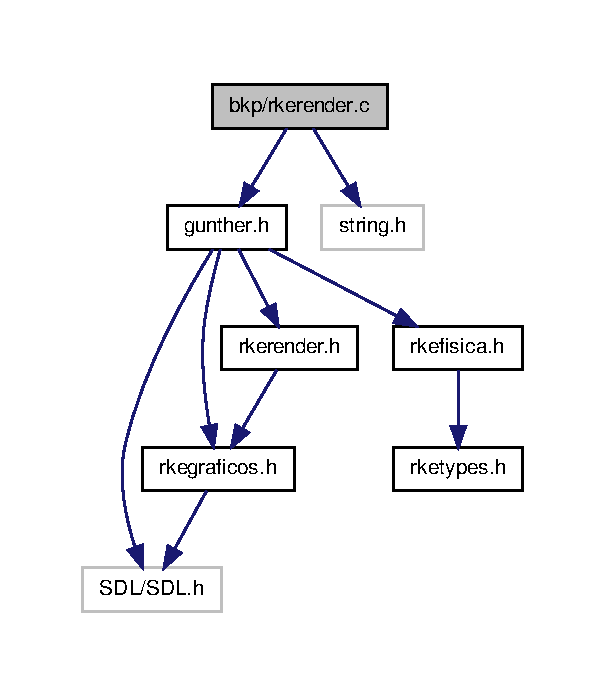
\includegraphics[width=291pt]{rkerender_8c__incl}
\end{center}
\end{figure}
\subsection*{Definições e Macros}
\begin{DoxyCompactItemize}
\item 
\hypertarget{rkerender_8c_abe0ec1d45aab5f79cf2ea355a5869890}{
\#define {\bfseries BOMBA}~1}
\label{rkerender_8c_abe0ec1d45aab5f79cf2ea355a5869890}

\item 
\hypertarget{rkerender_8c_a864ac6616dfea2db2da5fa7cb56bc814}{
\#define {\bfseries FLECHA}~0}
\label{rkerender_8c_a864ac6616dfea2db2da5fa7cb56bc814}

\end{DoxyCompactItemize}
\subsection*{Funções}
\begin{DoxyCompactItemize}
\item 
void \hyperlink{rkerender_8c_a239c7a748de2f7055719398fc04fe922}{rke\_\-render} (char $\ast$fase, char $\ast$imagens, char $\ast$img\_\-jogador, int largura, int altura, int larg\_\-ladrilho, int alt\_\-ladrilho)
\item 
void \hyperlink{rkerender_8c_a4fb57e2863d45d122b3cfa8b70a78aa9}{rke\_\-move\_\-jogador} (\hyperlink{struct__jogador}{Jogador} $\ast$jogador, \hyperlink{struct__tabuleiro}{Tabuleiro} tabuleiro, \hyperlink{struct__ladrilho}{Ladrilho} $\ast$terrenos, \hyperlink{struct__objeto}{Objeto} $\ast$objetos, int delta\_\-x, int delta\_\-y)
\item 
void \hyperlink{rkerender_8c_aa69f373b7090123c26ef782d099b9524}{rke\_\-jogador\_\-atira} (\hyperlink{struct__jogador}{Jogador} $\ast$jogador, \hyperlink{struct__tabuleiro}{Tabuleiro} tabuleiro, \hyperlink{struct__ladrilho}{Ladrilho} $\ast$terrenos, \hyperlink{struct__objeto}{Objeto} $\ast$objetos, int bomba)
\item 
int \hyperlink{rkerender_8c_a33b39c80a9bf85e9d591eae389194976}{rke\_\-acoes\_\-objetos} (\hyperlink{struct__jogador}{Jogador} $\ast$jogador, \hyperlink{struct__tabuleiro}{Tabuleiro} tabuleiro, \hyperlink{struct__ladrilho}{Ladrilho} $\ast$terrenos, \hyperlink{struct__objeto}{Objeto} $\ast$objetos)
\item 
void \hyperlink{rkerender_8c_a8dc5a9555b2b8a1e08c811a7a35469ea}{rke\_\-carrega\_\-terreno} (char $\ast$arquivo, \hyperlink{struct__ladrilho}{Ladrilho} terrenos\mbox{[}$\,$\mbox{]}, int larg\_\-ladrilho, int alt\_\-ladrilho)
\item 
void \hyperlink{rkerender_8c_af0f031a450b3be6ba5c5bc5b6d103653}{rke\_\-carrega\_\-objetos} (char $\ast$arquivo, \hyperlink{struct__objeto}{Objeto} objetos\mbox{[}$\,$\mbox{]}, int larg\_\-ladrilho, int alt\_\-ladrilho)
\item 
void \hyperlink{rkerender_8c_aaa263ecd9eccd396516779b7ef6710f6}{rke\_\-carrega\_\-fase} (char $\ast$arquivo, \hyperlink{struct__tabuleiro}{Tabuleiro} $\ast$tabuleiro, int $\ast$jogador\_\-x, int $\ast$jogador\_\-y)
\item 
void \hyperlink{rkerender_8c_a367aed7c3de5f557a25d934be4aee8a4}{rke\_\-carrega\_\-jogador} (\hyperlink{struct__jogador}{Jogador} $\ast$jogador, int larg\_\-ladrilho, int alt\_\-ladrilho)
\end{DoxyCompactItemize}


\subsection{Descrição Detalhada}
Renderizador de fases. \begin{DoxyAuthor}{Autor}
João da Silva, Marina Salles, Ricardo Macedo 
\end{DoxyAuthor}


\subsection{Funções}
\hypertarget{rkerender_8c_a33b39c80a9bf85e9d591eae389194976}{
\index{rkerender.c@{rkerender.c}!rke\_\-acoes\_\-objetos@{rke\_\-acoes\_\-objetos}}
\index{rke\_\-acoes\_\-objetos@{rke\_\-acoes\_\-objetos}!rkerender.c@{rkerender.c}}
\subsubsection[{rke\_\-acoes\_\-objetos}]{\setlength{\rightskip}{0pt plus 5cm}int rke\_\-acoes\_\-objetos (
\begin{DoxyParamCaption}
\item[{{\bf Jogador} $\ast$}]{jogador, }
\item[{{\bf Tabuleiro}}]{tabuleiro, }
\item[{{\bf Ladrilho} $\ast$}]{terrenos, }
\item[{{\bf Objeto} $\ast$}]{objetos}
\end{DoxyParamCaption}
)}}
\label{rkerender_8c_a33b39c80a9bf85e9d591eae389194976}
Função de acoes independentes dos objetos. 
\begin{DoxyParams}{Parâmetros}
{\em jogador} & Informações do jogador \\
\hline
{\em tabuleiro} & Informações do tabuleiro \\
\hline
{\em terrenos} & Informações dos elementos de terreno \\
\hline
{\em objetos} & Informações dos objetos \\
\hline
\end{DoxyParams}
\hypertarget{rkerender_8c_aaa263ecd9eccd396516779b7ef6710f6}{
\index{rkerender.c@{rkerender.c}!rke\_\-carrega\_\-fase@{rke\_\-carrega\_\-fase}}
\index{rke\_\-carrega\_\-fase@{rke\_\-carrega\_\-fase}!rkerender.c@{rkerender.c}}
\subsubsection[{rke\_\-carrega\_\-fase}]{\setlength{\rightskip}{0pt plus 5cm}void rke\_\-carrega\_\-fase (
\begin{DoxyParamCaption}
\item[{char $\ast$}]{arquivo, }
\item[{{\bf Tabuleiro} $\ast$}]{tabuleiro, }
\item[{int $\ast$}]{jogador\_\-x, }
\item[{int $\ast$}]{jogador\_\-y}
\end{DoxyParamCaption}
)}}
\label{rkerender_8c_aaa263ecd9eccd396516779b7ef6710f6}
Carrega as informações do tabuleiro da fase 
\begin{DoxyParams}{Parâmetros}
{\em arquivo} & O arquivo com as informações \\
\hline
{\em tabuleiro} & O lugar para armazenar as informações \\
\hline
{\em jogador\_\-x} & Argumento que devolve a posição X do jogador \\
\hline
{\em jogador\_\-y} & Argumento que devolve a posição Y do jogador \\
\hline
\end{DoxyParams}
\hypertarget{rkerender_8c_a367aed7c3de5f557a25d934be4aee8a4}{
\index{rkerender.c@{rkerender.c}!rke\_\-carrega\_\-jogador@{rke\_\-carrega\_\-jogador}}
\index{rke\_\-carrega\_\-jogador@{rke\_\-carrega\_\-jogador}!rkerender.c@{rkerender.c}}
\subsubsection[{rke\_\-carrega\_\-jogador}]{\setlength{\rightskip}{0pt plus 5cm}void rke\_\-carrega\_\-jogador (
\begin{DoxyParamCaption}
\item[{{\bf Jogador} $\ast$}]{jogador, }
\item[{int}]{larg\_\-ladrilho, }
\item[{int}]{alt\_\-ladrilho}
\end{DoxyParamCaption}
)}}
\label{rkerender_8c_a367aed7c3de5f557a25d934be4aee8a4}
Carrega os retângulos da imagem do jogador 
\begin{DoxyParams}{Parâmetros}
{\em O} & lugar para armazenar as informações \\
\hline
{\em Largura} & em pixels do ladrilho \\
\hline
{\em Altura} & em pixels do ladrilho \\
\hline
\end{DoxyParams}
\hypertarget{rkerender_8c_af0f031a450b3be6ba5c5bc5b6d103653}{
\index{rkerender.c@{rkerender.c}!rke\_\-carrega\_\-objetos@{rke\_\-carrega\_\-objetos}}
\index{rke\_\-carrega\_\-objetos@{rke\_\-carrega\_\-objetos}!rkerender.c@{rkerender.c}}
\subsubsection[{rke\_\-carrega\_\-objetos}]{\setlength{\rightskip}{0pt plus 5cm}void rke\_\-carrega\_\-objetos (
\begin{DoxyParamCaption}
\item[{char $\ast$}]{arquivo, }
\item[{{\bf Objeto}}]{objetos\mbox{[}$\,$\mbox{]}, }
\item[{int}]{larg\_\-ladrilho, }
\item[{int}]{alt\_\-ladrilho}
\end{DoxyParamCaption}
)}}
\label{rkerender_8c_af0f031a450b3be6ba5c5bc5b6d103653}
Carrega as informações dos objetos de um arquivo 
\begin{DoxyParams}{Parâmetros}
{\em arquivo} & O arquivo com as informações \\
\hline
{\em objetos} & O lugar para armazenar as informações \\
\hline
{\em larg\_\-ladrilho} & Largura em pixels do ladrilho \\
\hline
{\em alt\_\-ladrilho} & Altura em pixels do ladrilho \\
\hline
\end{DoxyParams}
\hypertarget{rkerender_8c_a8dc5a9555b2b8a1e08c811a7a35469ea}{
\index{rkerender.c@{rkerender.c}!rke\_\-carrega\_\-terreno@{rke\_\-carrega\_\-terreno}}
\index{rke\_\-carrega\_\-terreno@{rke\_\-carrega\_\-terreno}!rkerender.c@{rkerender.c}}
\subsubsection[{rke\_\-carrega\_\-terreno}]{\setlength{\rightskip}{0pt plus 5cm}void rke\_\-carrega\_\-terreno (
\begin{DoxyParamCaption}
\item[{char $\ast$}]{arquivo, }
\item[{{\bf Ladrilho}}]{terrenos\mbox{[}$\,$\mbox{]}, }
\item[{int}]{larg\_\-ladrilho, }
\item[{int}]{alt\_\-ladrilho}
\end{DoxyParamCaption}
)}}
\label{rkerender_8c_a8dc5a9555b2b8a1e08c811a7a35469ea}
Carrega as informações dos elementos de terreno de um arquivo 
\begin{DoxyParams}{Parâmetros}
{\em arquivo} & O arquivo com as informações \\
\hline
{\em terrenos} & O lugar para armazenar as informações \\
\hline
{\em larg\_\-ladrilho} & Largura em pixels do ladrilho \\
\hline
{\em alt\_\-ladrilho} & Altura em pixels do ladrilho \\
\hline
\end{DoxyParams}
\hypertarget{rkerender_8c_aa69f373b7090123c26ef782d099b9524}{
\index{rkerender.c@{rkerender.c}!rke\_\-jogador\_\-atira@{rke\_\-jogador\_\-atira}}
\index{rke\_\-jogador\_\-atira@{rke\_\-jogador\_\-atira}!rkerender.c@{rkerender.c}}
\subsubsection[{rke\_\-jogador\_\-atira}]{\setlength{\rightskip}{0pt plus 5cm}void rke\_\-jogador\_\-atira (
\begin{DoxyParamCaption}
\item[{{\bf Jogador} $\ast$}]{jogador, }
\item[{{\bf Tabuleiro}}]{tabuleiro, }
\item[{{\bf Ladrilho} $\ast$}]{terrenos, }
\item[{{\bf Objeto} $\ast$}]{objetos, }
\item[{int}]{bomba}
\end{DoxyParamCaption}
)}}
\label{rkerender_8c_aa69f373b7090123c26ef782d099b9524}
Função de acao de atirar do jogador. 
\begin{DoxyParams}{Parâmetros}
{\em jogador} & Informações do jogador \\
\hline
{\em tabuleiro} & Informações do tabuleiro \\
\hline
{\em terrenos} & Informações dos elementos de terreno \\
\hline
{\em objetos} & Informações dos objetos \\
\hline
\end{DoxyParams}
\hypertarget{rkerender_8c_a4fb57e2863d45d122b3cfa8b70a78aa9}{
\index{rkerender.c@{rkerender.c}!rke\_\-move\_\-jogador@{rke\_\-move\_\-jogador}}
\index{rke\_\-move\_\-jogador@{rke\_\-move\_\-jogador}!rkerender.c@{rkerender.c}}
\subsubsection[{rke\_\-move\_\-jogador}]{\setlength{\rightskip}{0pt plus 5cm}void rke\_\-move\_\-jogador (
\begin{DoxyParamCaption}
\item[{{\bf Jogador} $\ast$}]{jogador, }
\item[{{\bf Tabuleiro}}]{tabuleiro, }
\item[{{\bf Ladrilho} $\ast$}]{terrenos, }
\item[{{\bf Objeto} $\ast$}]{objetos, }
\item[{int}]{delta\_\-x, }
\item[{int}]{delta\_\-y}
\end{DoxyParamCaption}
)}}
\label{rkerender_8c_a4fb57e2863d45d122b3cfa8b70a78aa9}
Função de movimentação do jogador. 
\begin{DoxyParams}{Parâmetros}
{\em jogador} & Informações do jogador \\
\hline
{\em tabuleiro} & Informações do tabuleiro \\
\hline
{\em terrenos} & Informações dos elementos de terreno \\
\hline
{\em objetos} & Informações dos objetos \\
\hline
{\em delta\_\-x} & Movimentação no eixo X \\
\hline
{\em delta\_\-y} & Movimentação no eixo Y \\
\hline
\end{DoxyParams}
\hypertarget{rkerender_8c_a239c7a748de2f7055719398fc04fe922}{
\index{rkerender.c@{rkerender.c}!rke\_\-render@{rke\_\-render}}
\index{rke\_\-render@{rke\_\-render}!rkerender.c@{rkerender.c}}
\subsubsection[{rke\_\-render}]{\setlength{\rightskip}{0pt plus 5cm}void rke\_\-render (
\begin{DoxyParamCaption}
\item[{char $\ast$}]{fase, }
\item[{char $\ast$}]{imagens, }
\item[{char $\ast$}]{img\_\-jogador, }
\item[{int}]{largura, }
\item[{int}]{altura, }
\item[{int}]{larg\_\-ladrilho, }
\item[{int}]{alt\_\-ladrilho}
\end{DoxyParamCaption}
)}}
\label{rkerender_8c_a239c7a748de2f7055719398fc04fe922}
Função principal do renderizador de fases 
\begin{DoxyParams}{Parâmetros}
{\em fase} & Arquivo de fase \\
\hline
{\em imagens} & Arquivo clipboard com as imagens para terreno e objetos \\
\hline
{\em img\_\-jogador} & Arquivo clipboard com as imagens do jogador \\
\hline
{\em largura} & Largura em ladrilhos da tela \\
\hline
{\em altura} & Altura em ladrilhos da tela \\
\hline
{\em larg\_\-ladrilho} & Largura em pixels do ladrilho \\
\hline
{\em alt\_\-ladrilho} & Altura em pixels do ladrilho \\
\hline
\end{DoxyParams}

\printindex
\end{document}
